\documentclass[12pt,a4paper,abstract=on,bibliography=totoc]{scrartcl}
\usepackage{cite}
\usepackage{amsmath}
\usepackage{hyperref}
\usepackage{subfigure}
\usepackage{graphicx}
\usepackage{listings}
\usepackage{lmodern}
\usepackage{amsfonts}
\usepackage{algorithm,algorithmic}
\usepackage[swedish,english]{babel}
\lstset{
    language=python,
    breaklines=true,
    showspaces=false,
    showstringspaces=false,
    frame=single,
    basicstyle=\footnotesize\ttfamily,
    keywordstyle=\color{blue}\bfseries,
    stringstyle=\color[rgb]{0.6,0.1,0.1},
    commentstyle=\color{purple},
    numbers=left
}

\title{Reinforcement learning for robotic manipulation}
\subtitle{Master thesis}
\author{Isac Arnekvist \\ \texttt{isacar@kth.se} \\ KTH Robotics Perception and Learning lab \\ Supervisor: Johannes A. Stork}

\begin{document}
\maketitle
\begin{abstract}

Reinforcement learning was recently successfully used for real-world robotic
manipulation tasks, without the need for human demonstration, using a
\textit{normalized advantage function}-algorithm (NAF). Limitations on the
shape of the advantage function however poses doubts to what kind of policies
can be learned using this method. For similar tasks, convolutional neural
networks have been used for pose estimation from images taken with
fixed-position cameras. For some applications however, this might not be a
valid assumption. It was also shown that the quality of policies for robotic
tasks severely deteriorates from small camera offsets. NAF is in this thesis
successfully used to solve simple tasks on real robotic systems where data
collection is distributed over several robots, and learning is done on a
separate server.  Using NAF to learn a pushing task, with clear multi-modal
properties, however fails to converge to a good policy, both on the real robots
and in simulation. Deep deterministic policy gradient (DDPG) is instead used
in simulation and successfully learns to solve the task. The learned policy is
then applied on the real robots and accomplishes to solve the task in the real
setting as well. Pose estimation from fixed position camera images is learned
and the policy is still able to solve the task using these estimates. By
defining a coordinate frame from an object visible to the camera, in this case
the robot arm, a neural network learns to regress the pushable objects pose in
this frame without the assumption of a fixed camera. However, the precision of
the predictions were too inaccurate to be used for solving the pushing task.
Further modifications to this approach could however show to be a feasible
solution to randomly placed cameras with unknown poses.

\end{abstract}


\begin{otherlanguage}{swedish}
    \begin{abstract}

        Reinforcement learning har nyligen använts framgångsrikt för att lära
        icke-simulerade robotar uppgifter med hjälp av en \textit{normalized
        advantage function}-algoritm (NAF), detta utan att använda mänskliga
        demonstrationer.  Restriktioner på funktionsytorna som använts kan dock
        visa sig vara problematiska för generalisering till andra uppgifter.
        För pose-estimering har i liknande sammanhang convolutional neural
        networks använts med bilder från kamera med konstant position. I vissa
        applikationer kan dock inte kameran garanteras hålla en konstant
        position och studier har visat att kvaliteten på policys kraftigt
        förvärras när kameran förflyttas. NAF appliceras i denna uppsats
        framgångsrikt på enklare problem där datainsamling är distribuerad över
        flera robotar och inlärning sker på en central server. Vid applicering
        på en uppgift med tydliga multimodala egenskaper misslyckas dock NAF.
        Deep deterministic policy gradient (DDPG) appliceras istället på
        problemet och lär sig framgångsrikt att lösa problemet i simulering.
        Den inlärda policyn appliceras sedan framgångsrikt på riktiga robotar.
        Pose-estimering genom att använda en fast kamera implementeras också
        framgångsrikt. Genom att definiera ett koordinatsystem från ett föremål
        i bilden med känd position, i detta fall robotarmen, kan andra föremåls
        positioner beskrivas i denna koordinatram med hjälp av neurala nätverk.
        Dock så visar sig precisionen vara för låg för att appliceras på
        robotar. Resultaten visar ändå att denna metod, med ytterligare
        utökningar och modifikationer, skulle kunna lösa problemet.

    \end{abstract}
\end{otherlanguage}

\tableofcontents
\section{Introduction}

\subsection{Robotic manipulation}

Reinforcement Learning (RL) deals with learning what actions to do in order to
reach a long-term goal (a \textit{policy} is learned) and have been widely used
for learning robotic manipulation tasks. Recent research suggests methods
capable of learning real-world robotic manipulation tasks without simulation
pre-training, learning only from real-world experience
\cite{yahya2016collective,gu2016deep,finn2016deep,chebotar2016path}. Using
visual feedback for manipulation tasks is a way to handle unknown poses of
manipulators and target objects and training these kind of tasks end-to-end
have been successful in simulation tasks
\cite{schulman2015trust,lillicrap2015continuous}. Real-world manipulation tasks
have also been learned with visual feedback but using pre-trained pose
estimation networks \cite{gu2016deep}. Pose estimation have been shown to work
by using convolutional neural networks (CNN)
\cite{levine2016end,chebotar2016path,yahya2016collective}, although for some
cases it was shown that test-time translations severely effected manipulation
task performance \cite{yahya2016collective}. CNNs have been trained to deal
with relative poses \cite{park20163d}, and this could be a feasible solution to
deal with unknown random camera offsets. Real-world experiments often rely on
human demonstrations to learn a successful policy but this might not always be
available. Recently a successful demonstration of learning a door opening task
from scratch without the need for human demonstration or simulation
pre-training have been shown \cite{gu2016deep}. This was using a version of
Normalized Advantage Function algorithms (NAF) \cite{gu2016continuous}
distributed over several robotic platforms.

\subsection{This study}

A series of experiments were conducted in order to verify the distributed
version of NAF in new contexts. Relatively inexpensive robotic
cartesian-controlled arms were used for pushing objects into randomly sampled
poses. To further extend previous results \cite{gu2016deep}, pose estimation
was done using a CNN in accordance with previous work
\cite{levine2016end,chebotar2016path,yahya2016collective}. It was further
evaluated whether training the pose estimation network with randomly placed
camera positions could make it more robust to translations.

\subsection{Motivation}

Positive results could imply further automation of manipulation tasks where
relative poses of robots, sensors, and targets are unknown. Using a CNN that
estimates relative poses and that is robust to translations could be
interesting also for researchers and industry beyond the robotics use case as
in this thesis.

\section{Related work}

Concepts and vocabulary used here assume previous knowledge of RL and neural
networks. These concepts are more thoroughly described in the background
section, section \ref{sec:background}.

\subsection{Normalized Advantage Functions (NAF)}

In order to extend Q-learning, normally used for discrete state and action
spaces to continuous spaces, Gu et al. \cite{gu2016continuous} proposes a
relatively simple solution called normalized advantage functions (NAF). They
argue after doing simulation experiments that this algorithm is an effective
alternative to recently proposed actor-critic methods and that it learns faster
with more accurate resulting policies. First, the action-value function is
divided into a sum of the value function $V$ and what they call an advantage
function $A : \mathbb{R}^d \longmapsto \mathbb{R}$:

\begin{equation}
    Q(\mathbf{x}, \mathbf{u}) = A(\mathbf{x}, \mathbf{u}) + V(\mathbf{x})
\end{equation}

Here, $\mathbf{x}$ is the state of the environment and $\mathbf{u}$ are
controls or actions. The advantage function is a quadratic function of $u$:

\begin{equation}
    A(\mathbf{x}, \mathbf{u}) = -\frac{1}{2}(\mathbf{u} - \mathbf{\mu(x)})^T\mathbf{P(x)}(\mathbf{u} - \mathbf{\mu(x)})
    \label{eq:advantage_function}
\end{equation}

There are more terms that need to be defined, but first consider equation
(\ref{eq:advantage_function}). The matrix $\mathbf{P}$ is a positive-definite
matrix, this makes the advantage function have its maximum when $\mathbf{u =
\mu(x)}$.  The purpose of $\mu$ is to be a greedy policy function, thus
$\mathbf{Q}$ is maximized when $\mathbf{u}$ is the greedy action. The purpose
of this is that given an optimal $Q$, we do not need to search for the optimal
action, since we know $\mathbf{\mu}$. Now the definition of $\mathbf{P}$:

\begin{equation}
    P(\mathbf{x}) = \mathbf{L(x)L(x)}^T
\end{equation}

Here, $\mathbf{L}$ is a lower-triangular matrix where diagonal entries are
strictly positive.

After these definitions, we are left with estimating the functions $V$,
$\mathbf{\mu}$, and $\mathbf{L}$. To this end the authors use a neural network,
here shown in figure \ref{fig:naf-net}. The $\mathbf{L}$ output is fully
connected with the previous layer and not passed through an activation function
(it is linear). The diagonal entries of L are exponentiated. Hidden layers
consisted of 200 fully connected units with rectified linear units (ReLU) as
activation functions except for $\mathbf{L}$ and $A$ as already defined.

\begin{figure}[h]
    \centering
    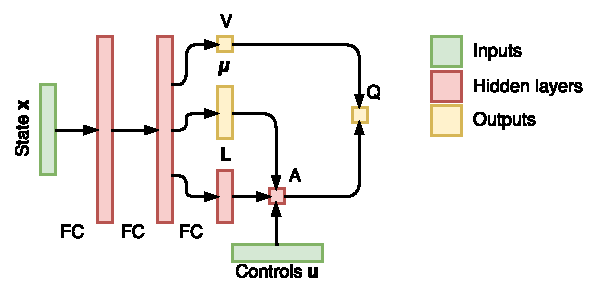
\includegraphics[width=1.0\textwidth]{res/naf-net.pdf}

    \caption{Neural network design for NAF \cite{gu2016continuous}. The
    activation function to $V$ was not specified. The tanh activation was added
    in figure due to Gu et al. \cite{gu2016deep} using it in order to have
    bounded actions for safety reasons.}

    \label{fig:naf-net}
\end{figure}

The NAF algorithm is listed in algorithm \ref{algo:naf}. All collected experiences
are stored in a replay buffer that optimization is run against. Exploration is done
by adding noise to the current greedy policy $\mathbf{\mu}$.

\begin{algorithm}[!h]
    \caption{NAF algorithm}
    \begin{algorithmic}
        \STATE{Randomly initialize network $Q(x, u|\theta)$}
        \STATE{Initialize target network $Q'$, $\theta' \leftarrow \theta$}
        \STATE{Initialize replay buffer $R \leftarrow \emptyset$}
        \FOR{episode $= 1$ to $M$}
            \STATE{Initialize random process $\mathcal{N}$ for action exploration}
            \STATE{Receive initial exploration state $x_1$}
            \FOR{$t = 1$ to $T$}
                \STATE{Select action $\mathbf{u_t = \mu(x_t|\theta) + \mathcal{N}_t}$}
                \STATE{Execute $\mathbf{u_t}$ and observe $r_t$ and $\mathbf{x}_{t+1}$}
                \STATE{Store transition $(\mathbf{x}_t, \mathbf{u}_t, r_t, \mathbf{x}_{t+1})$ in $R$}
                \FOR{iteration $= 1$ to $I$}
                    \STATE{Sample a random minibatch of $m$ transitions from $R$}
                    \STATE{Set $y_i = r_i + \gamma V'(\mathbf{x}_{i+1}|\theta')$}
                    \STATE{Update $\theta$ by minimizing the loss:
                           $L = \frac{1}{N}\sum_i (y_i - Q(\mathbf{x}_i, \mathbf{u}_i|\theta))^2$}
                    \STATE{Update target network $\theta' \leftarrow \tau \theta + (1 - \tau)\theta'$}
                \ENDFOR
            \ENDFOR
        \ENDFOR
    \end{algorithmic}
    \label{algo:naf}
\end{algorithm}

\subsection{Distributed real-world learning using NAF}
\label{sec:distributed_naf}

Real-world experiments were done by Gu et al. \cite{gu2016deep} on door opening
tasks using the NAF algorithm and 7-DoF torque controlled arms. They extended
the algorithm to be distributed on several robots/collectors and one separate
trainer thread on a separate machine. They state that this was the first
successful real-world experiment with a relatively high complexity problem
without human demonstration or simulated pretraining. They used the layout of
the network shown in figure \ref{fig:naf-net} but with hidden layers of 100
units each. Also, in this article it was explicitly mentioned that the
activation functions for the policy $\mathbf{\mu}$ was tanh in order to bound
the actions. The state input consisted of the arm pose and target pose. The
target pose was known from attached equipment. The modified version of NAF is
listed in algorithm \ref{algo:async_naf}.

The authors conclude that there was an upper bound on the effects of
parallelization, but hypothesize that the speed of the trainer thread has a
limiting factor in this matter. They used CPU for training the neural network
so instead using a GPU might increase the effect of more collectors.

\begin{algorithm}[!h]
    \caption{Asynchronous NAF - $N$ collector threads and $1$ trainer thread}
    \begin{algorithmic}
        \STATE{// trainer thread}
        \STATE{Randomly initialize network $Q(\mathbf{x}, \mathbf{u}|\theta)$}
        \STATE{Initialize target network $Q'$, $\theta' \leftarrow \theta$}
        \STATE{Initialize shared replay buffer $R \leftarrow \emptyset$}
        \FOR{iteration $= 1$ to $I$}
            \STATE{Sample a random minibatch of m transitions from $R$}
            \STATE{Set $y_i = \begin{cases}r_i+\gamma V'(x_i|\theta) &\text{ if } t_i < T,\\r_i &\text{ if } t_i = T\end{cases}$}
            \STATE{Update $\theta$ by minimizing the loss:
                   $L = \frac{1}{m} \sum_i (y_i - Q(\mathbf{x}_i, \mathbf{u}_i|\theta))^2$}
            \STATE{Update the target network: $\theta' \leftarrow \tau\theta + (1-\tau)\theta'$}
        \ENDFOR
        \STATE{// collector thread $n$, $n = 1...N$}
        \FOR{episode $= 1$ to $M$}
            \STATE{Sync policy network weights $\theta_n \leftarrow \theta$}
            \STATE{Initialize a random process $\mathcal{N}$ for action exploration}
            \STATE{Receive initial observation state $x_1$}
            \FOR{$t = 1$ to $T$}
                \STATE{Select action $\mathbf{u}_t = \mathbf{mu}$}
                \STATE{Execute $\mathbf{u}_t$ and observe $r_t$ and $\mathbf{x}_{t+1}$}
                \STATE{Send transition $(\mathbf{x}_t, \mathbf{u}_t, r_t, \mathbf{x}_{t+1}, t)$ to $R$}
            \ENDFOR
        \ENDFOR
    \end{algorithmic}
    \label{algo:async_naf}
\end{algorithm}

\subsection{Spatial softmax in pose estimation}

Levine et al. \cite{levine2016end} proposed an architecture for a CNN that
gives pose estimates for robotic manipulation tasks. After the last
convolutional layer, a softmax is applied, but only normalized over each
kernel's response map, called \textit{spatial softmax}:

\begin{equation}
    s_{cij} = \frac{e^{a_{cij}}}{\sum_{i',j'} e^{a_{ci'j'}}}
\end{equation}

Here, $a_{cij}$ is the output of the $c$:th kernel at coordinate $ij$. After
this, they calculate the expected 2D position for each feature, which they
argue is better suited for pose estimation. The expected 2D position is
expressed as a tuple $(f_{cx}, f_{cy})$ calculated according to:

\begin{align}
    f_{cx} &= \sum_{i,j} s_{ij} x_{ij} \\
    f_{cy} &= \sum_{i,j} s_{ij} y_{ij}
\end{align}

The scalar value $x_{ij}$ is the position in image space of the pixel at coordinate
$(i, j)$. This can reasonably easy be simplified to a matrix multiplication with constant
weights from each of the response maps. Arguably, it could also be possible to rewrite the
above expressions as:

\begin{align}
    f_{cx} &= \sum_{i,j} i s_{ij} \\
    f_{cy} &= \sum_{i,j} j s_{ij}
\end{align}

\subsection{Door opening with human demonstration}

Chebotar et al. \cite{chebotar2016path} demonstrates door opening tasks
initialized from human demonstration using methods called Guided Policy Search
(GPS) and Policy Improvement with Path Integrals (PI$^2$). They demonstrate
that they can learn this task outputting torque control from visual input. This is
extended by Yahya et al. \cite{yahya2016collective} to be trained
simultaneously on several robots. In both cases, torque commands are the output
of a neural network where the first part takes visual input and is pretrained
with pose estimates of the door and the robot arm. This neural network is shown
in figure \ref{fig:gps_net}. Since the robot poses were labeled in the robot
base frame and the camera offsets were somewhat random, a linear mapping from
the neural network output to the base frame was learned separately for each of
the robots. The authors evaluated the trained policy on a previously unseen
door with different translations and rotations. The mean success rate was
90\%. They also tried offsetting the camera 1) 5 cm towards the ground and 2) 4
cm backwards. The respective success rates for these translations were 52 \%
and 54 \%.

\begin{figure}[h]
    \centering
    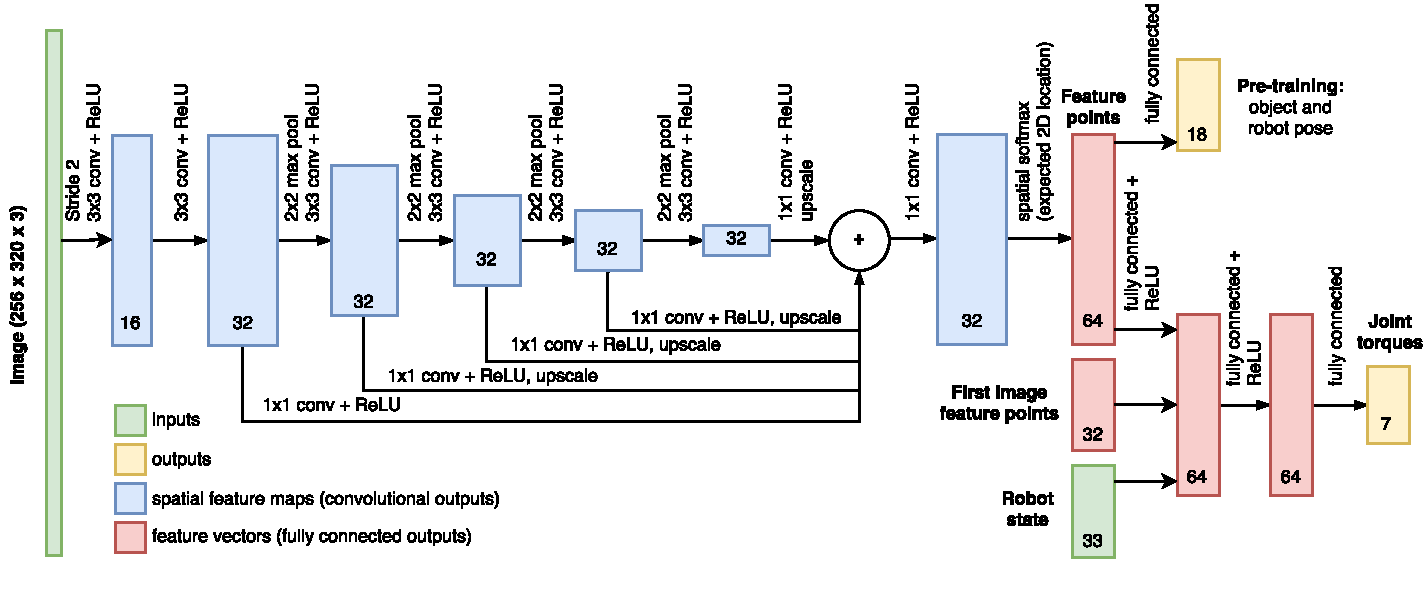
\includegraphics[width = 1.0\textwidth]{res/gps-net.pdf}
    \caption{Network used for door opening task from visual inputs \cite{chebotar2016path}}
    \label{fig:gps_net}
\end{figure}

\subsection{Prioritized experience replay}
\label{sec:prio_sampling}

When randomly sampling experiences from a replay buffer, one alternative is to
sample from a uniform distribution. However, if samples are sampled from a
distribution where experiences with larger temporal-difference errors are more
likely to be chosen, training times can be reduced with resulting policies that
outperform those trained by uniform sampling \cite{schaul2015prioritized}. Let
$R_{t}$ be the reward at time $t$, $Q(S_t, A_t)$ the Q-function of state $S_t$
and action $A_t$ at time $t$ and $V(S_t)$ the value function for $S_t$ at time
$t$. Given a sample tuple $x_i = (S_t, S_{t+1}, A_t, R_{t+1})$, let the
temporal-difference error for this sample to be defined as:

\begin{equation}
    \delta_i = Q(S_{t}, A_t) - \left[ R_{t+1} + \gamma V(S_{t+1}) \right]
\end{equation}

Define a priority $p_i$ of sample $x_i$ as:

\begin{equation}
    p_i = |\delta_i| + \epsilon
\end{equation}

Here $\epsilon > 0$ ensures all priorities are strictly positive. Sample experiences
according to the probability:

\begin{equation}
    P(i) = \frac{p_i^\alpha}{\sum_k p_k^\alpha}
\end{equation}

The hyperparameter $\alpha \geq 0$ enforces more uniform probabilities for values close to
zero and more non-uniform probabilities for larger values.

Since the gradient is biased by a biased choice of samples, the magnitude of
the gradient with respect to each sample $x_i$ can be weighted by:

\begin{equation}
    w_i = \left( \frac{1}{P(i)} \right)^\beta
\end{equation}

The parameter $\beta \geq 0$ can be varied during training, and it is argued that
the unbiased gradients are more important towards the end when the policy is
converging. They varied this parameter reaching $\beta = 1$ only towards the
end of the training. It is not clear from the article but it is assumed that
training starts with $\beta = 0$.

\subsection{Adam}
\cite{kingma2014adam}

%\subsection{Motion planning by a predictive model}
%
%Another method for learning manipulation tasks was shown by Finn and Levine
%\cite{finn2016deep}. Given a sequence of initial images, they denote it
%$I_{0:1}$, together with robot poses $x_{0:1}$, and future commands $a_{1:H_p}$
%where $H_p$ is some prediction horizon, they predict the distribution of future
%images $I_{2:H_p + 1}$. $I_t$ is here a collection of independent pixel
%distributions with mean $\hat{I}_t$. A convolutional LSTM was used for this,
%and an implicit feature of the network is what they call a flow map
%$\hat{F}_t(x, y, k, l)$ which is the probability of the pixel at coordinates
%$(k, l)$ at time $t+1$ originating from coordinates $(x, y)$. Given a flow map
%they can do one step prediction:
%
%\begin{equation}
%    \hat{F}_t \odot \hat{I}_t := \sum_{k \in (-\kappa, \kappa)} \sum_{l \in (-\kappa, \kappa)} \hat{F}_t(x,y,k,l)\hat{I}_t(x-k, y-l) = \hat{I}_{t+1}
%\end{equation}
%
%When using these implicit flow operators rather than actual predicted image
%which was the output from the network, they can predict movement of individual
%pixels for several time steps ahead. Using a maximum likelihood approach, they
%can find the series of actions that puts a pixel at some other target location.
%For evaluation, they try their trained algorithm on previously unseen objects
%by selecting start and end coordinates for which it generalized.
%
%An interesting feature of their approach is that the data set for training was
%generated by torque-controlled arms randomly interacting with a collection of
%objects and recording images of it along with the robot poses. Therefore, no
%part of the training needed human supervision or demonstration. Another feature
%is that the camera positions were not the same across robots, it is unclear if
%they evaluated the method with a new camera position though.
%

\section{Background}

\subsection{Objective}

The interest in conducting this thesis research started with a series of
articles published by researchers at Google in their research blog
\cite{gu2016deep,finn2016deep,yahya2016collective,chebotar2016path}. The main
theme in these articles was robotic manipulation learned by gathering
experience in real time in non-simulated contexts. These articles will be
presented in more detail below and extended during the pilot study. In two of
these articles \cite{gu2016deep,finn2016deep} tasks are learned from scratch
without the need for initializing by demonstration. Although, in the article by
Gu et al. \cite{gu2016deep}, poses of targets and arms are known by attached
equipment. It would be interesting to incorporate estimation of poses from
visual feedback in this case to lessen the need for external equipment. Another
central theme in these articles is the distributed collection of experience
over several robots. This is done in order to decrease the time it takes to
collect data and to increase variance of the data. The use cases for
incorporating and extending these findings could be robotic manipulation tasks
with camera as feedback where exact relative positions of objects,
manipulators, and sensors need not be fixed. Also, where resources exists to
use several robots for speeding up the learning process. Possible readers might
be other researchers working with end-to-end machine learning for robotic
manipulation. Other interested parties might also be manufacturers where
repetitive tasks are a part of the production chain and variations in these
make it hard for robots to be easily programmed for those tasks.

\subsection{Reinforcement learning}

This entire section is a descriptions of key concepts from a book on
Reinforcement Learning by Sutton and Barto \cite{sutton1998reinforcement}.

\subsubsection{The three tiers of machine learning}

In reinforcement learning (RL) an agent interacts with an environment and tries
to maximize some \textit{reward}, or rather the total amount of reward received
over time. To maximize the reward in the long run might require short-time
losses, making the problem more complex than just maximizing for one step at a
time.  To find a good strategy, commonly referred to as a \textit{policy}, the
agent uses its experience to make better decisions, this is referred to as
\textit{exploitation}. But, it must also find a balance between exploitation
and to also try out new things, i. e. \textit{exploration}. These things are
specific for RL and therefore distinguishes it from supervised and unsupervised
learning making it a third piece of machine learning.

\subsubsection{Main elements of RL}

A policy is a function from the state of the environment to an action, i. e.
the function that chooses what to do under any state. A reward is an immediate
signal given by the environment that the agent receives after each interaction.
Since a reward is only short-term a \textit{value function} tries to estimate
the total amount of reward that will be given in the long run when taking some
action. To enable planning of actions in the environment, RL algorithms
sometimes uses a \textit{model} in order to try out actions in this before
making decisions. This is usually referred to as model-based RL in contrast to
model-free.

\subsubsection{Finite Markov Decision Processes}

In a RL scenario where the environment has a finite number of states, there is
a finite number of actions, and the Markov property holds is called a
\textit{finite Markov Decision Process} (finite MDP). Let $S_t$ be the state at
time $t$, $R_t$ be the reward at time $t$, and $A_t$ the action at time $t$.
The interaction between an agent and its environment in RL is that the agent at
each time step $t$ reads the environment and takes an action. The environment
changes, maybe stochastically, by responding with a new state and a reward at
time $t+1$. The dynamics of a finite MDP is completely specified by the
probability distribution:

\begin{equation}
    p(s', r|s, a) = P(S_{t+1} = s', R_{t+1} = r | S_t = s, A_t = a)
\end{equation}

State-value function (TODO: define $\gamma$ and purpose, define/skip $G$ also?):
\begin{equation}
    v_\pi(s) = \mathbb{E}_\pi\left[G_t|S_t=s\right] = \mathbb{E}_\pi\left[\sum_{k=0}^\infty \gamma^k R_{t+k+1}|S_t=s\right]
\end{equation}

Action-value function:
\begin{equation}
    q_\pi(s, a) = \mathbb{E}_\pi\left[G_t|S_t=s,A_t=a\right] = \mathbb{E}_\pi\left[\sum_{k=0}^\infty \gamma^k R_{t+k+1}|S_t=s,A_t=a\right]
\end{equation}


\subsubsection{Q-Learning}
TODO: Mention somewhere \textit{on-policy} and \textit{off-policy}.
\begin{equation}
    Q(S_t, A_t) \leftarrow Q(S_t, A_t) + \alpha \left[ R_{t+1} + \gamma \max_a Q(S_{t+1}, a) - Q(S_t, A_t) \right]
\end{equation}

\subsection{Pilot study}

The following sections are the preliminary sources of information that was the
initial spark for this thesis as mentioned above. How to re-implement these
articles is not self-contained, so the pilot would necessarily need to also
include reading into articles from the references of these. Reading of these
initial articles would be needed to motivate an appropriate method, and then
further research would be done with the purpose of gaining all the information
needed to implement such a solution. The thesis study will be conducted at the
Robotics, Perception, and Learning lab at KTH with the main interest originally
being to dig into these articles and develop something further.

\subsubsection{Motion planning by ''Deep visual foresight''}

This article \cite{finn2016deep} trains a convolutional neural network on
images together with motion as inputs to predict how the image will change due
to that motion. This is later used to plan movement of objects to some target
pose.

\subsubsection{Path Integral Guided Policy Search}

In this article \cite{chebotar2016path}, the authors extend Guided Policy
Search and demonstrate two manipulation tasks. These are initialized from
demonstrations. To be able to comprehend this article, referenced articles
\cite{levine2016end,theodorou2010generalized,montgomery2016guided} would have
to be read as well.

\subsubsection{Collective Robot Reinforcement Learning with Distributed
               Asynchronous Guided Policy Search}

This article \cite{yahya2016collective} distributes learning of
door opening across several robots. The exact nature of the tasks
are varied across robots to increase robustness. The learning is
initialized from demonstration.

\subsubsection{Parallelized training without prior demonstration}

This article \cite{gu2016deep} shows several robotic manipulation tasks where
learning is parallelized across platforms, and they do not require previous
demonstrations.  For this article, I would need to read up on an algorithm
called Normalized Advantage Function (NAF) \cite{gu2016continuous}. In both of
the two previously mentioned articles
\cite{chebotar2016path,yahya2016collective} pose estimation of targets and
robots are done through visual feedback, while in this article
\cite{gu2016deep} no sensory feedback is provided and poses are known through
attached equipment. The pose estimation was done using a convolutional neural
network which could be a feasible extension to this article.


\subsubsection{Reinforcement learning}

These articles mentioned above naturally deals with reinforcement vocabulary
and assumes knowledge in this area. Therefore the pilot would include studying
a book by Sutton and Barto \cite{sutton1998reinforcement}. In this book,
chapters 1-3 and a section about non-linear function approximators are
essential (by advice from supervisor).

\subsection{Problem statement}

Manipulation tasks that seem trivial to a human can be hard to learn for
robots, especially from scratch without initial human demonstration due to high
sample complexity. Recent research suggests ways to do this but are based on
that you know the poses of the objects and the end-effector. For some scenarios
these are non-trivial to find out.

Problems also arise when learning in real time by collecting experience. Robots
must be able to evaluate their policies regularly at a high rate which is
complicated by adding a deep convolutional neural network for pose detection.
Also, learning tasks within a feasible time frame is harder when data
collection and policy updates happen in real time. The approach of
distributing collection of experience over several robots will be evaluated in
this thesis for handling this problem.

\subsection{Research question}

How can deep and distributed reinforcement learning be used for learning and
performing dynamic manipulation tasks with unknown poses.

\subsection{Expected scientific results}

If all goes well, previous results are verified in new contexts. Also
they are extended to also handle unknown target and manipulator poses.


\chapter{Method}

\section{The task and partial goals}

The final goal, or task, to accomplish was pushing a cube from and to some
arbitrary positions in the workspace of the robot. The task was researched
using a reinforcement learning approach, only specifying the wanted behavior by
defining a reward function $f(s, a, s') \in \mathbb{R}$, where $s, a, s'$ is
the state, action, and successor state. The state here includes the robot and
cube state along with the goal. First-order Markov property is assumed together
with assuming the state as observable, formulating the problem as a Markov
Decision Process (MDP).

An iterative approach was taken in order to solve the task, starting by solving
simpler tasks before increasing the complexity. This way algorithms are sanity
checked in a natural fashion and making limitations of model formulations
clearer as complexity is added. The first task was to investigate appending
arbitrary goals to the state for a reaching task with a simulated agent and
environment. This was later extended to being trained on data from distributed
real robotic systems. Pushing tasks were then attempted in simulation followed
by evaluating trained policies on real robots. As a second part to this thesis,
pose estimation from camera was researched with the goal to relax the
assumption of a fixed position camera or known offset to the camera. This was
also done in an iterative fashion starting with a fixed position camera and
then using simulations to investigate neural network capabilities given perfect
features. Finally, trained pose estimation models were evaluated on the real
robotic systems, replacing pose estimates from other sensors.

\section{Robotic environment}
\label{sec:robo_env}

Low cost robotic arms (uArm Metal) were used along with a dedicated computer,
and a \textit{LIght Detection And Range}-device (LIDAR) for pose estimation of
the cube. For pose estimation from camera, an RGB-camera with an optional
RGB-aligned depth channel was used. A workspace for the entire setup was
defined to be $x \in [-0.1, 0.1]$, $y \in [0.1, 0.3]$ (meters), both for the
reaching and pushing task. The coordinate frame used is shown in figure
\ref{fig:workspace_lidar_place} (top left), along with the placement of the
LIDAR and camera (top right).

\begin{figure}[h]
    \centering
    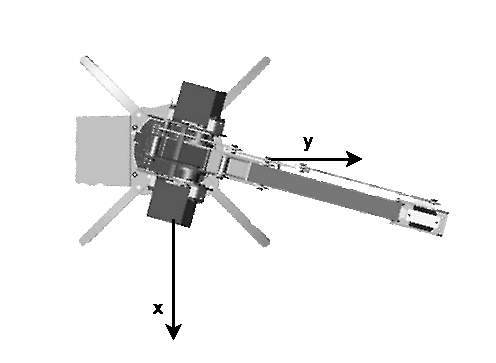
\includegraphics[width=0.50 \textwidth]{res/uarm_coordinates.pdf}
    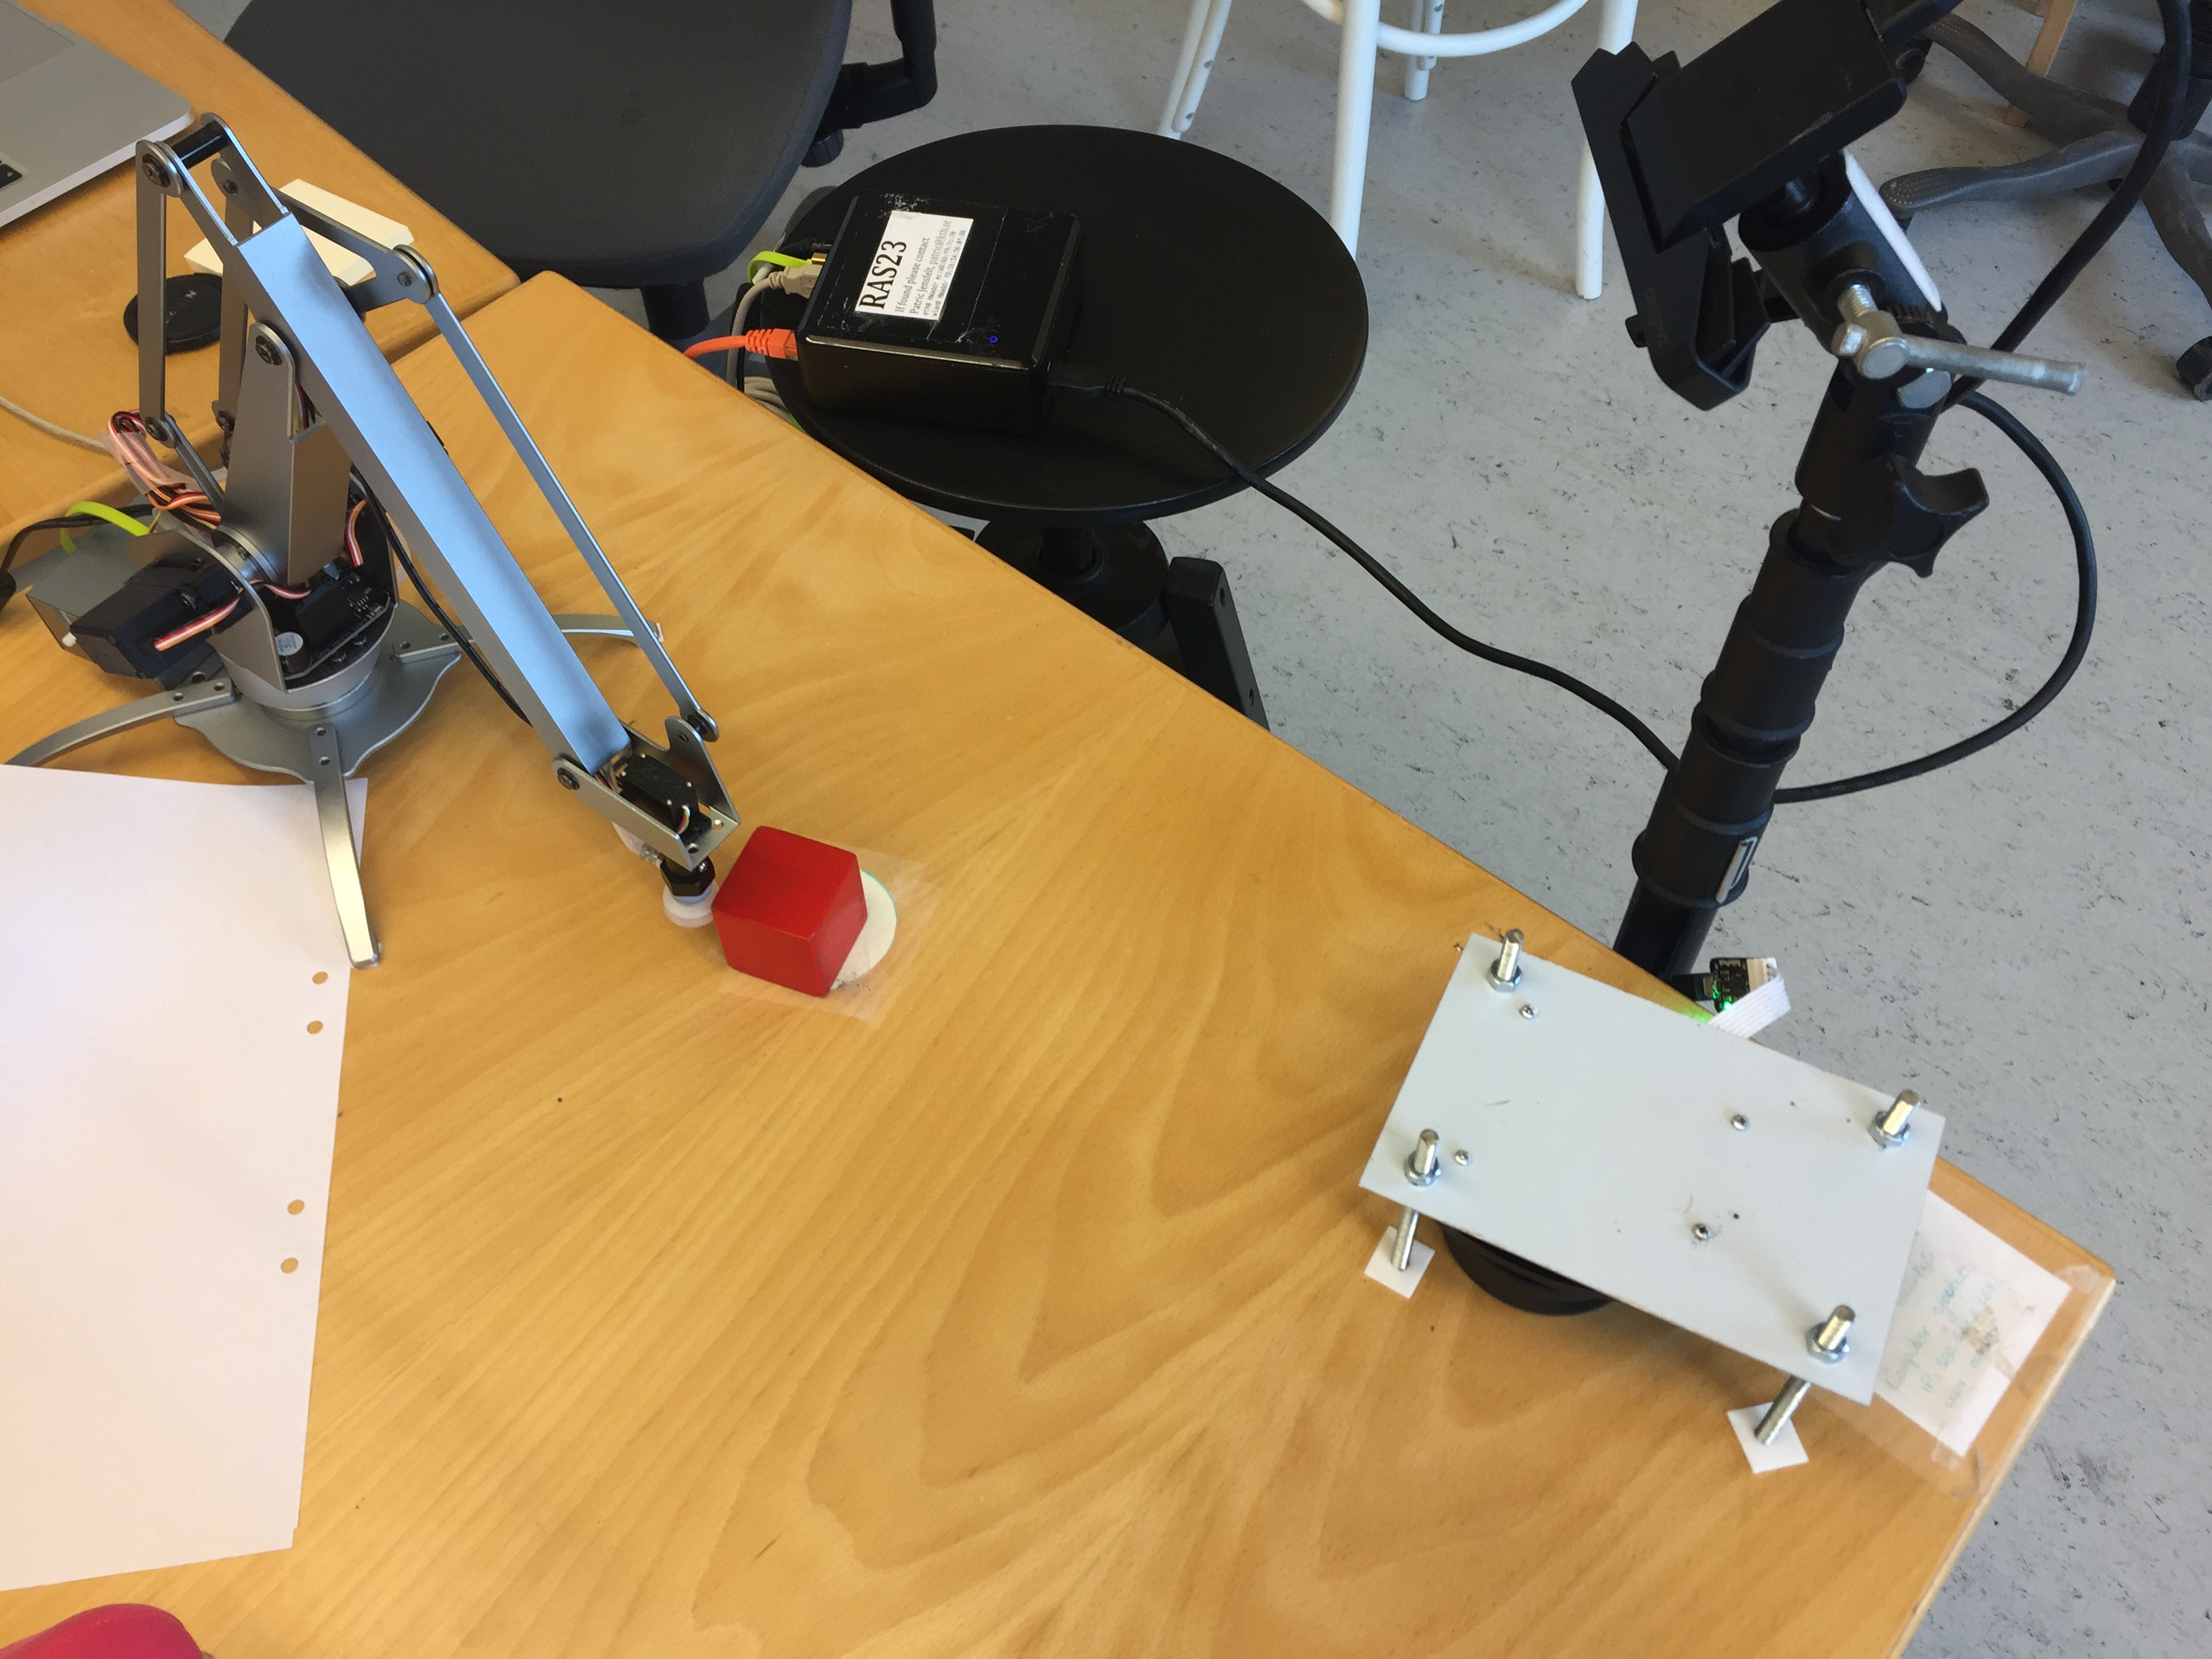
\includegraphics[width=0.49 \textwidth]{res/camera_placement_fixed.jpg}
    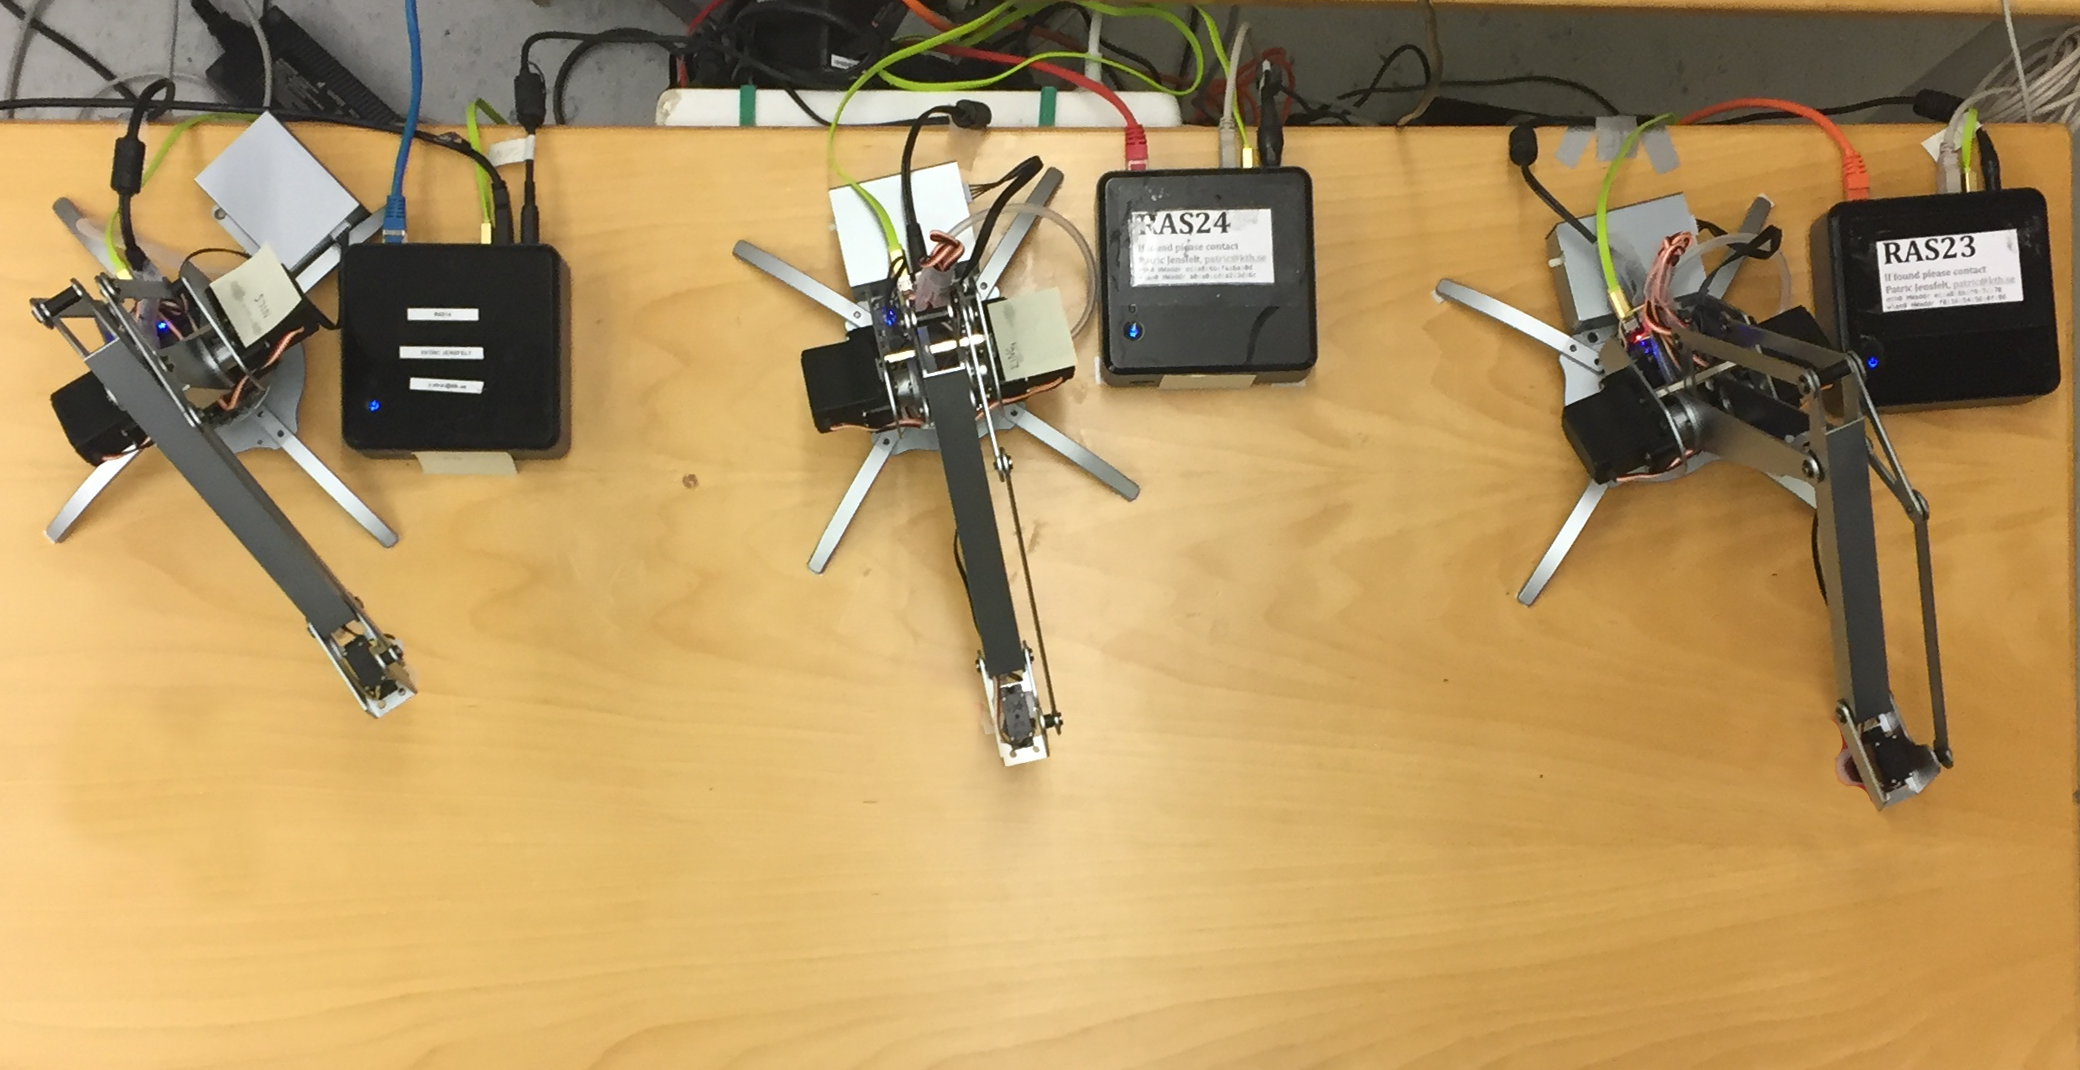
\includegraphics[width=1.00 \textwidth]{res/uarm_moving_setup.png}

    \caption{Top left: Coordinate frame used for the robot. Top right:
    Placement of the LIDAR, seen attached to a gray housing in the bottom right
    corner. The housing was built in order to mount the LIDAR such that it only
    registers reflecting light from the cube. The fixed camera position for
    cube pose estimation can also be seen in the top right corner of this picture.
    Bottom: For distributing data collection, several setups, each with a
    dedicated computer, was used.}

    \label{fig:workspace_lidar_place}

\end{figure}

The arms were in this thesis controlled by commanding servo angles, with an
implemented controller on top that could command the end-effector to some
cartesian coordinates. The arms have 4 degrees of freedom, but only three were
used in this thesis, ignoring the end-effector rotation servo. The arms were
shipped with controllers and forward/inverse kinematics but were not reliable,
therefore a new derivation of the kinematics was done along with a new
controller implementation.

\subsection{Inverse kinematics derivation}

Definition of landmarks and distances can be seen in figure
\ref{fig:uarm_landmarks}. We are given the coordinates of the point $D$ and
want to find to angles $\alpha$, $\beta$, and $\theta$.

\begin{figure}[!ht]
    \centering
    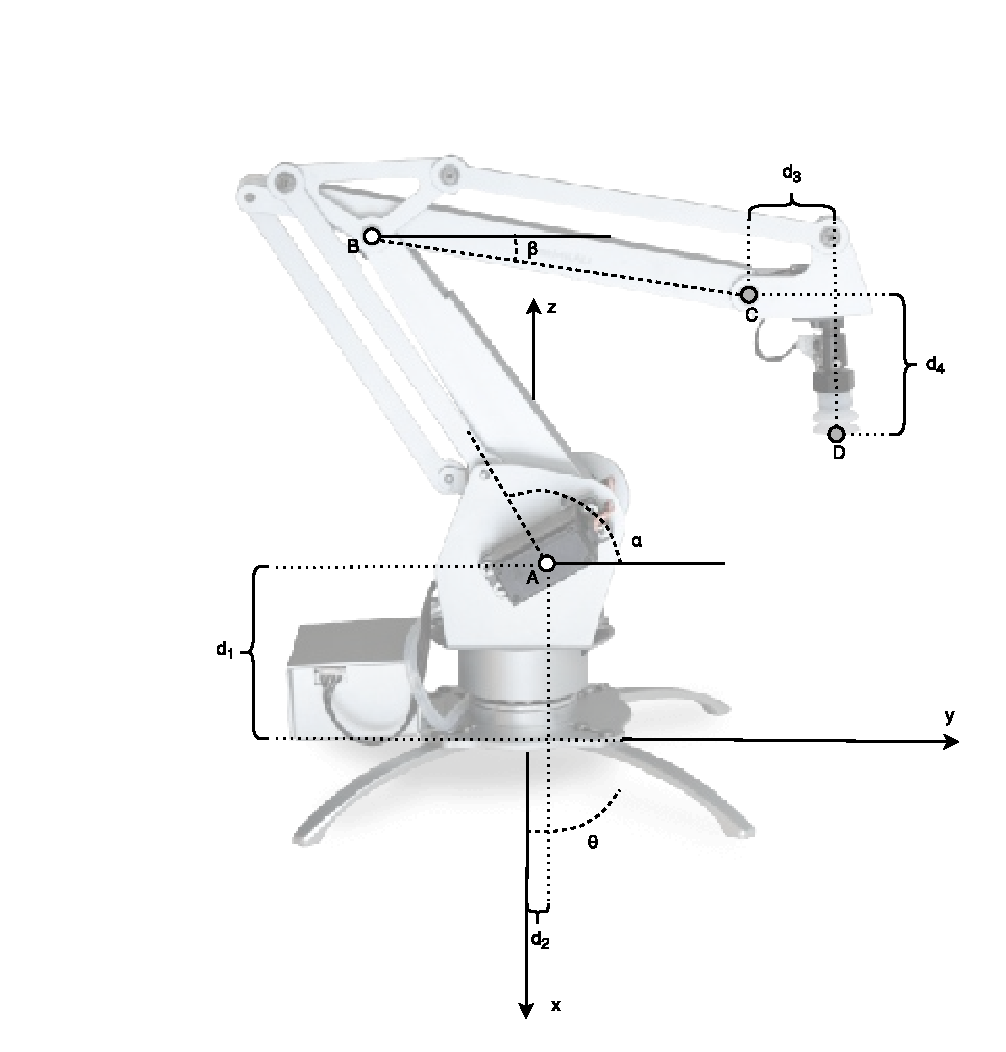
\includegraphics[width=0.80 \textwidth]{res/inverse_kinematics.pdf}

    \caption{Notation for landmarks used in derivation of inverse kinematics. A
    simplified problem is to consider the angles of the triangle $ABC$.}

    \label{fig:uarm_landmarks}

\end{figure}

The angle $\theta$ of the bottom servo that rotates the arm around the z-axis
is first simply found by:

\begin{equation}
    \theta = \text{arctan2}(y, x)
\end{equation}

The problem can then be simplified by only considering the 2D plane defined by
the points $A, B, C$, where the origin is placed at $A$.  Denote the
coordinates of $C$ in this new frame as:

\begin{equation}
    r = \sqrt{x^2 + y^2} - d_2 - d_3
\end{equation}

\begin{equation}
    h = z - d_1 - d_4
\end{equation}

Distances $d_{AB}$ and $d_{BC}$ are known constants, $d_{AC}$ is simply
$\sqrt{r^2 + h^2}$. Define the part of the $\alpha$ angle pointing towards
$C$ from $A$ as $\gamma$. This is found by:

\begin{equation}
    \gamma = \text{arctan2}(h, r)
\end{equation}

All sides of the triangle $ABC$ are known, so the angles are found by the rule (applied in the same fashion to all angles):

\begin{equation}
    \cos(BAC) = \frac{d_{AB}^2 + d_{AC}^2 - d_{BC}^2}{2 d_{AB} d_{AC}}
\end{equation}

The angle $\alpha$ is found by:

\begin{equation}
    \alpha = BAC + \gamma
\end{equation}

The angle between the vertical line going down from $A$ and $AB$ is $\alpha - \frac{\pi}{2}$
which implies:

\begin{equation}
    \beta = \frac{\pi}{2} - ABC - (\alpha - \frac{\pi}{2}) = \pi - ABC - \alpha
\end{equation}

\section{Simulated environment}
\label{sec:method_simulated}

A simple 2D environment was implemented with a circular pushable object, and a
point-like manipulator. Actions were sent to the environment as relative
movement of the manipulator. The environment does not take friction into
account, only moving the pushable object the minimum distance such that the
manipulator never exists within the object boundaries. Positions of goal,
manipulator, and object could be sampled according to different sampling
strategies, in the full problem each position is sampled uniformly within the
workspace. Samples of this environment is shown in figure
\ref{fig:env_sim_samples}. After each interaction, the environment returns
successor state and reward. For reaching tasks in simulation, the pushable
object is simply ignored.

\begin{figure}[!ht]
    \centering
    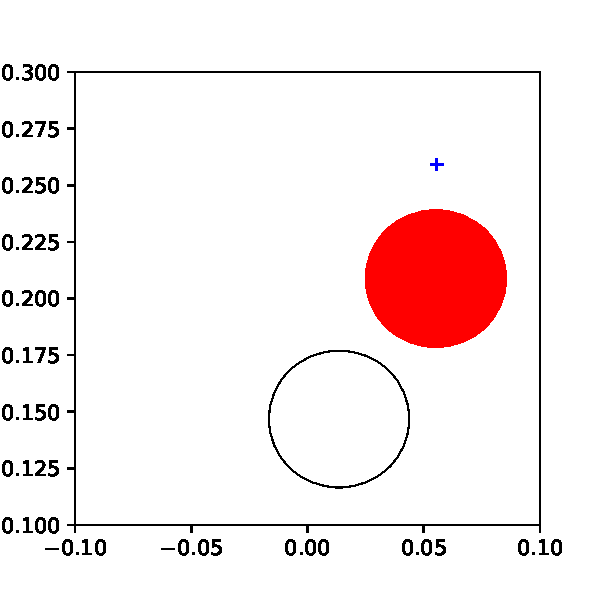
\includegraphics[width=0.3\textwidth]{res/env_sim1.pdf}
    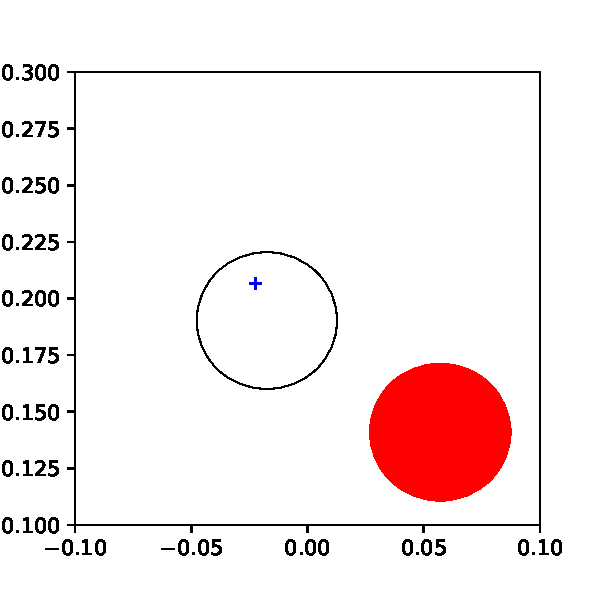
\includegraphics[width=0.3\textwidth]{res/env_sim2.pdf}
    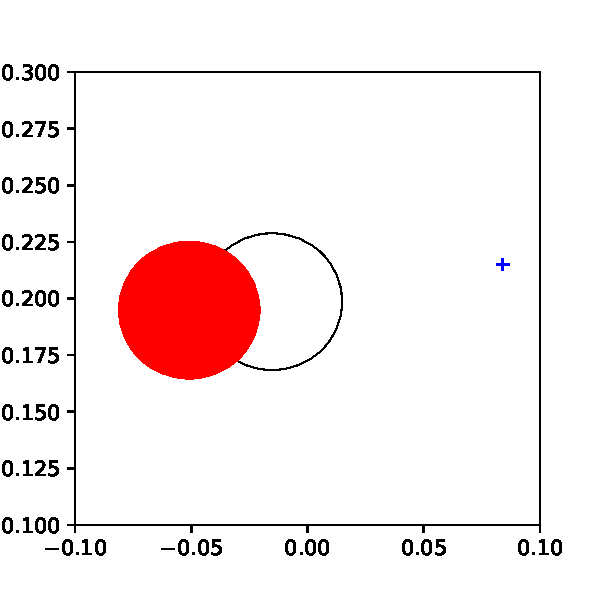
\includegraphics[width=0.3\textwidth]{res/env_sim3.pdf}

    \caption{The simulated environment for pushing, the cross represents the
    robot end-effector, red circle the pushable object, and the black/white
    circle the goal position.}

    \label{fig:env_sim_samples}
\end{figure}

\section{Estimating the cube position using LIDAR}
\label{sec:method_hough}

A LIDAR was used to estimate the position of the cube. These estimates were
both used as ground truth for training pose estimation neural networks, and
used as a part of the state for the reinforcement learning algorithms. The
LIDAR gives $360$ distance measurements at approximately evenly spaced angles,
with the angles having some variation from sweep to sweep. By sweep here is
meant a new set of 360 measurements from a full rotation of the laser. Sweeps
are returned at $10$ Hz. Only scans inside the defined workspace (section
\ref{sec:robo_env}) were considered for pose estimation of the cube. Only the
cube is assumed to reflect light from the LIDAR, the end-effector of the robot
was placed at a z-coordinate such that it is above the plane of the
LIDAR-scans.

To estimate the cube pose, the Hough-transform was used \cite{duda1972use}.
This algorithm takes as input a 2D matrix and returns scalar values for a set
of angles and distances $\lbrace \theta_1, ..., \theta_M\rbrace \times \lbrace
d_1, ..., d_N \rbrace$ each defining a line in the plane, see figure
\ref{fig:hough}. A large scalar for some $\theta_i$ and $d_i$ means that the
matrix entries along the coordinates specified by these parameters have higher
values, i.e. pixels form a line along the parameterized line.

\begin{figure}[h]
    \centering
    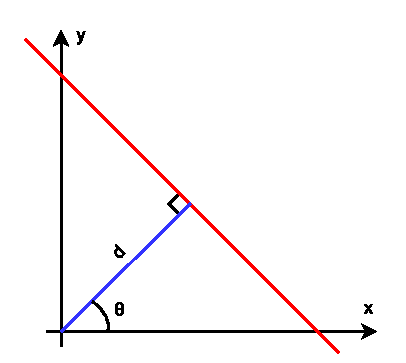
\includegraphics[width=0.39\textwidth]{res/hough.pdf}
    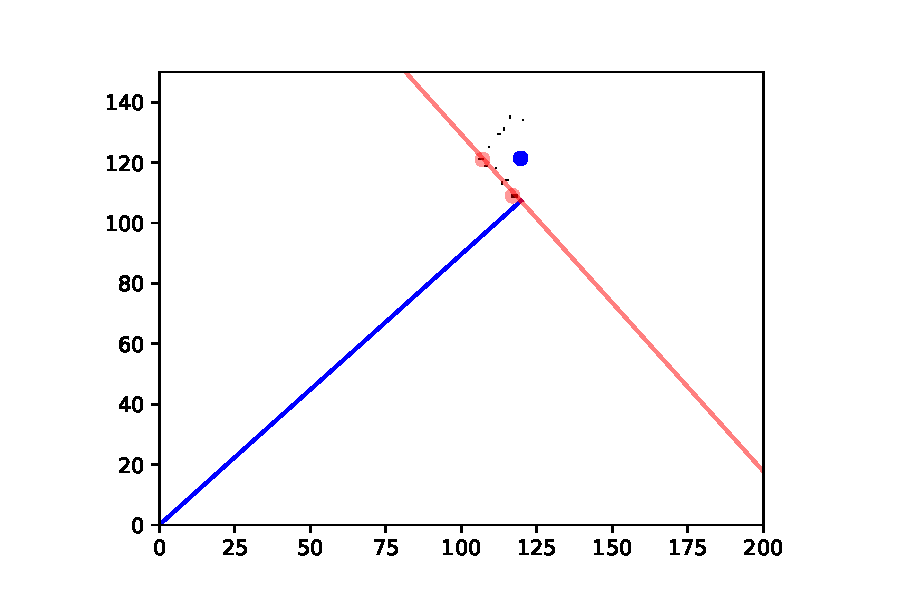
\includegraphics[width=0.60\textwidth]{res/hough_example.pdf}

    \caption{Left: The Hough transform returns scalar values for a set of lines each
    parameterized by some $\theta$ and $d$. In this figure the red line is
    parameterized by the angle $\theta$ and distance $d$.
    Right: LIDAR scans are plotted onto a binary matrix. The parameters with
    the maximum output from the Hough transform corresponds to the red line.
    The side of the cube is estimated by taking the outermost scans
    approximately lying on this line. The center of the cube is then found by
    adding an orthogonal vector from the center of this side with length
    corresponding to half of the cube size.}

    \label{fig:hough}
\end{figure}

The angles with corresponding distance measures from the LIDAR are converted to
cartesian space and plotted as ones onto a matrix of zeros (Hough transform
input), an example is shown in figure \ref{fig:hough} where the black pixels
correspond to LIDAR scans. After applying the transform on this image, the line
with the highest corresponding scalar value is chosen, in figure
\ref{fig:hough} shown as the red line. One of the cube's sides can then be
estimated using this line, limited by the outermost scans lying approximately
on this line, see red dots in figure \ref{fig:hough}. The center of the cube,
which is $4\times 4\times 4$ cm, is then estimated by adding the orthogonal
vector of length $2$ cm from the center of the estimated cube side (shown as
blue dot). Only the center of the cube was used for the experiments, although
the full pose of the cube is easily inferred from the found line.

The scans from the LIDAR showed variation between sweeps resulting in
variations in the pose estimates. This can be seen in figure
\ref{fig:lidar_noise}. The noise being relatively large imposes difficulties in
training policies using this data, and also for training neural network pose
estimators using LIDAR estimates as ground truth. Averaging estimates is one
solution to lowering errors but implies slower updates of the pose estimation.

\begin{figure}[h]
    \centering
    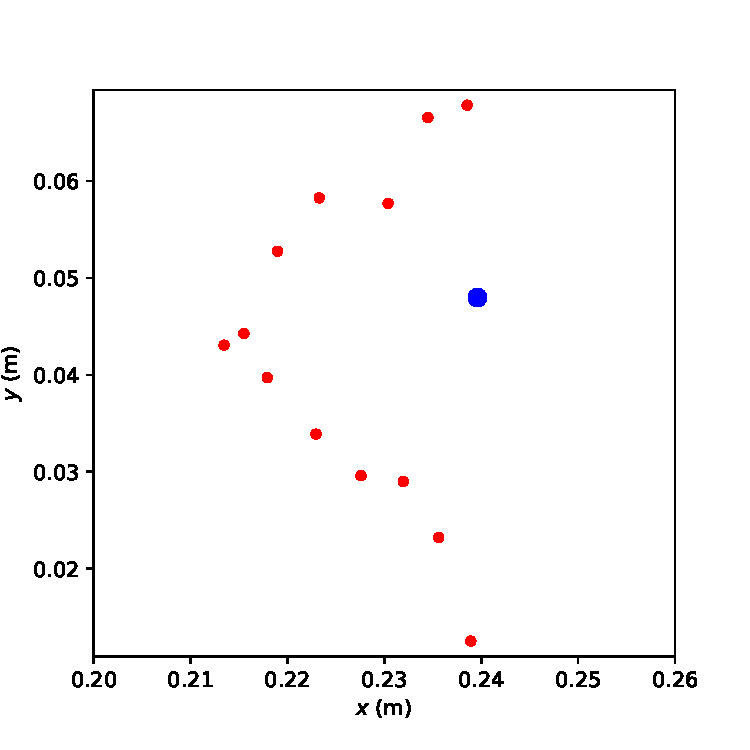
\includegraphics[width=0.49\textwidth]{res/cube_pose_lidar_one_scan.pdf}
    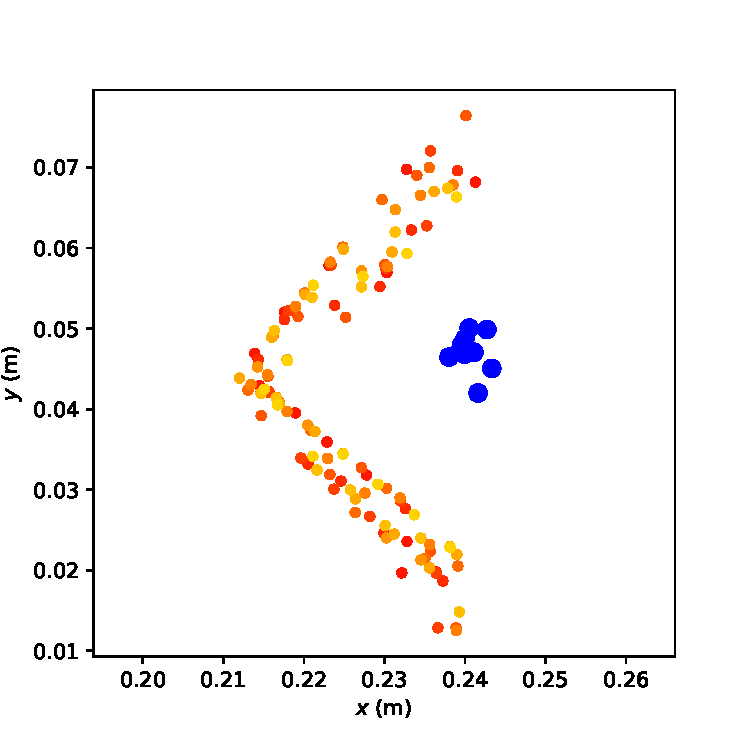
\includegraphics[width=0.49\textwidth]{res/cube_pose_lidar_variance.pdf}

    \caption{LIDAR scans (red) on a cube with the corresponding position
    estimate (blue). To the left one single sweep with the LIDAR clearly
    showing noisy measurements. To the right, plotting consecutive scans for
    the same cube position along with cube pose estimates shows noisy
    measurements and also noisy pose estimates of the cube. The different
    colors of the scans to the right represent different sweeps and show that
    the noise does not have a bias that is unique to the current sweep.}

    \label{fig:lidar_noise}
\end{figure}

\section{Software and libraries}

For high-level computational graphs, Keras \cite{chollet2015keras} was used.
For lower-level extensions not supported by Keras, Theano was used
\cite{theano2016theano}. For image pre-processing, plotting, and overall linear
algebra and mathematical computations, SciPy was used \cite{scipy2016scipy}.


\chapter{Reaching I: Simulated reaching task}

The pushing task defined puts no assumption on a constant goal position, rather
this should be able to be put randomly within the workspace. By appending the
goal position as part of the state, theoretically the goal could be constantly
moving and the policy should adjust accordingly. To investigate whether a
neural network easily can represent this policy, experiments were first
performed where the target is to reach randomly set goal positions with the
end-effector. If this cannot be accomplished in simulation, it is unlikely to
be accomplished on a real robotic system. The task was therefore learned in a
simulated environment first. The NAF algorithm was used since it showed
promising results on the real world door opening task without the need for
human demonstrations, and it has a straightforward way of distributing it
should it succeed.

\section{Method}

\subsection{Definition of the MDP}

The set of states

\begin{equation}
    \mathcal{S} \subset \mathbb{R}^2 \times \mathbb{R}^2
\end{equation}
is the cartesian product of end-effector end goal positions. The set of actions
\begin{equation}
    \mathcal{A} = \lbrace \mathbf{a} \in \mathbb{R}^2 \mid ||\mathbf{a}|| < 0.05 \rbrace
\end{equation}
is interpreted as the relative movement of the end-effector, although the
resulting position might vary due to a stochastic environment. The dynamics is
most succinctly described in two parts, the first part being the function
giving a successor end-effector position $\mathbf{e}'$ given previous position
$\mathbf{e}$ and action $\mathbf{a}$:
\begin{equation}
    \mathbf{e}' = \epsilon(\mathbf{e} + a), \epsilon \sim \mathcal{N}(1, 0.1^2)
\end{equation}
The goal $\mathbf{g}$ is constant during an episode which for formal
completeness is stated:
\begin{equation}
    \mathbf{g}' = \mathbf{g}
\end{equation}
The reward is a function of the successor state
\begin{equation}
    r(\mathbf{e', g'}) =
    \begin{cases}
        -2 &\text{if } \mathbf{e'} \text{ outside workspace}\\
        \exp\left(-k||\mathbf{e'} - \mathbf{g'}||^2\right) - 1 &\text{otherwise}
    \end{cases}
\end{equation}
Setting $k = 1000$ makes the reward equal $0$ close to the goal and rapidly
decay to $-1$ further from the goal. The value of $k$ was chosen to be $1000$
because it was seen, by plotting the reward function, to be large enough to
create a clear peak at the goal position, and small enough to avoid having
close-to-zero gradients of the reward function at other positions in the
workspace.
The discount factor $\gamma$ was defined to be equal to $0.98$.

\subsection{Environment}

A very simple simulated environment was used, as described in section
\ref{sec:method_simulated}, here ignoring the pushable object. This leaves only
workspace boundaries, and an end-effector that can be controlled by 2D
cartesian relative movements. The environment capped commands with norm larger
than $5$ cm. Commands were, in the environment, multiplied by Gaussian noise
$\mathcal{N}(1, 0.1^2)$ according the MDP definition, and the environment was
reset when reaching the outside the workspace or getting within a $1$ cm radius
of the goal. When resetting the environment, end-effector and goal poses were
randomly sampled within the workspace. The goal pose remained the same until
the environment was reset.

\subsection{Algorithms}

A NAF neural network was implemented with the same layout as described in
section \ref{sec:distributed_naf} with two hidden layers of $100$ units each.
The two dimensional $\mathbf{\mu}$ output had a $\tanh$ function scaled by
$0.05$ as activation. These  action outputs are not strictly correct according
to the above definition of the MDP, but this parameterization made more sense
than for example using polar coordinates. All poses were 2D where end-effector
and goal pose were concatenated as input to the network. A discount factor of
$0.98$ was used and the Adam optimizer \cite{kingma2014adam} was used with
learning rate $0.0001$ and a batch size of $512$. The replay buffer was sampled
from as described in section \ref{sec:prio_sampling} with $\alpha = 1$ and
$\beta$ in iteration $i$ out of a total amount of iterations $i_{tot}$ was set
according to:

\begin{equation}
    \beta_i = \exp \left( 10(i - i_{tot}) / i_{tot}\right)
\end{equation}

For sampling from the replay buffer, a binary tree was used where the value of
a parent equals the sum of its children \cite{schaul2015prioritized}. This way,
drawing one sample from a total of $N$ samples is $\mathcal{O}(\log_2(N))$. The
exact procedure is to first draw a sample from $U(0, \sum_i p_i)$ and then
start from the top of the tree and recurse down to the corresponding leaf node.
The loss was defined as the mean square error of the temporal-difference
errors. The training process was alternating between generating new experiences
by interacting with the environment, and between sampling batches from the
replay buffer to optimize the neural network. Explicit criterion for a
successful policy were not defined, rather training was run until plots of the
policy showed to move the end-effector towards the goal position from all
directions.

\section{Results}

The algorithm was running for approximately one hour collecting $\approx 100k$
state transitions. The learned policy and value functions are shown in figure
\ref{fig:sim_moving_goal}. The implementation, using the NAF formulation,
clearly solves the task and is able to handle changing goal positions given as
a part of the state. The value function estimates where less peaky around the
goal position than expected, but has to do with the formulation of the reward.
The reward being calculated from successor states, and a single action allowing
the agent to move $5$ cm, gives a plateau of approximately $5$ cm around the
goal from where the goal, and the maximum immediate reward, is reachable within
one action.

\begin{figure}[h]
    \centering
    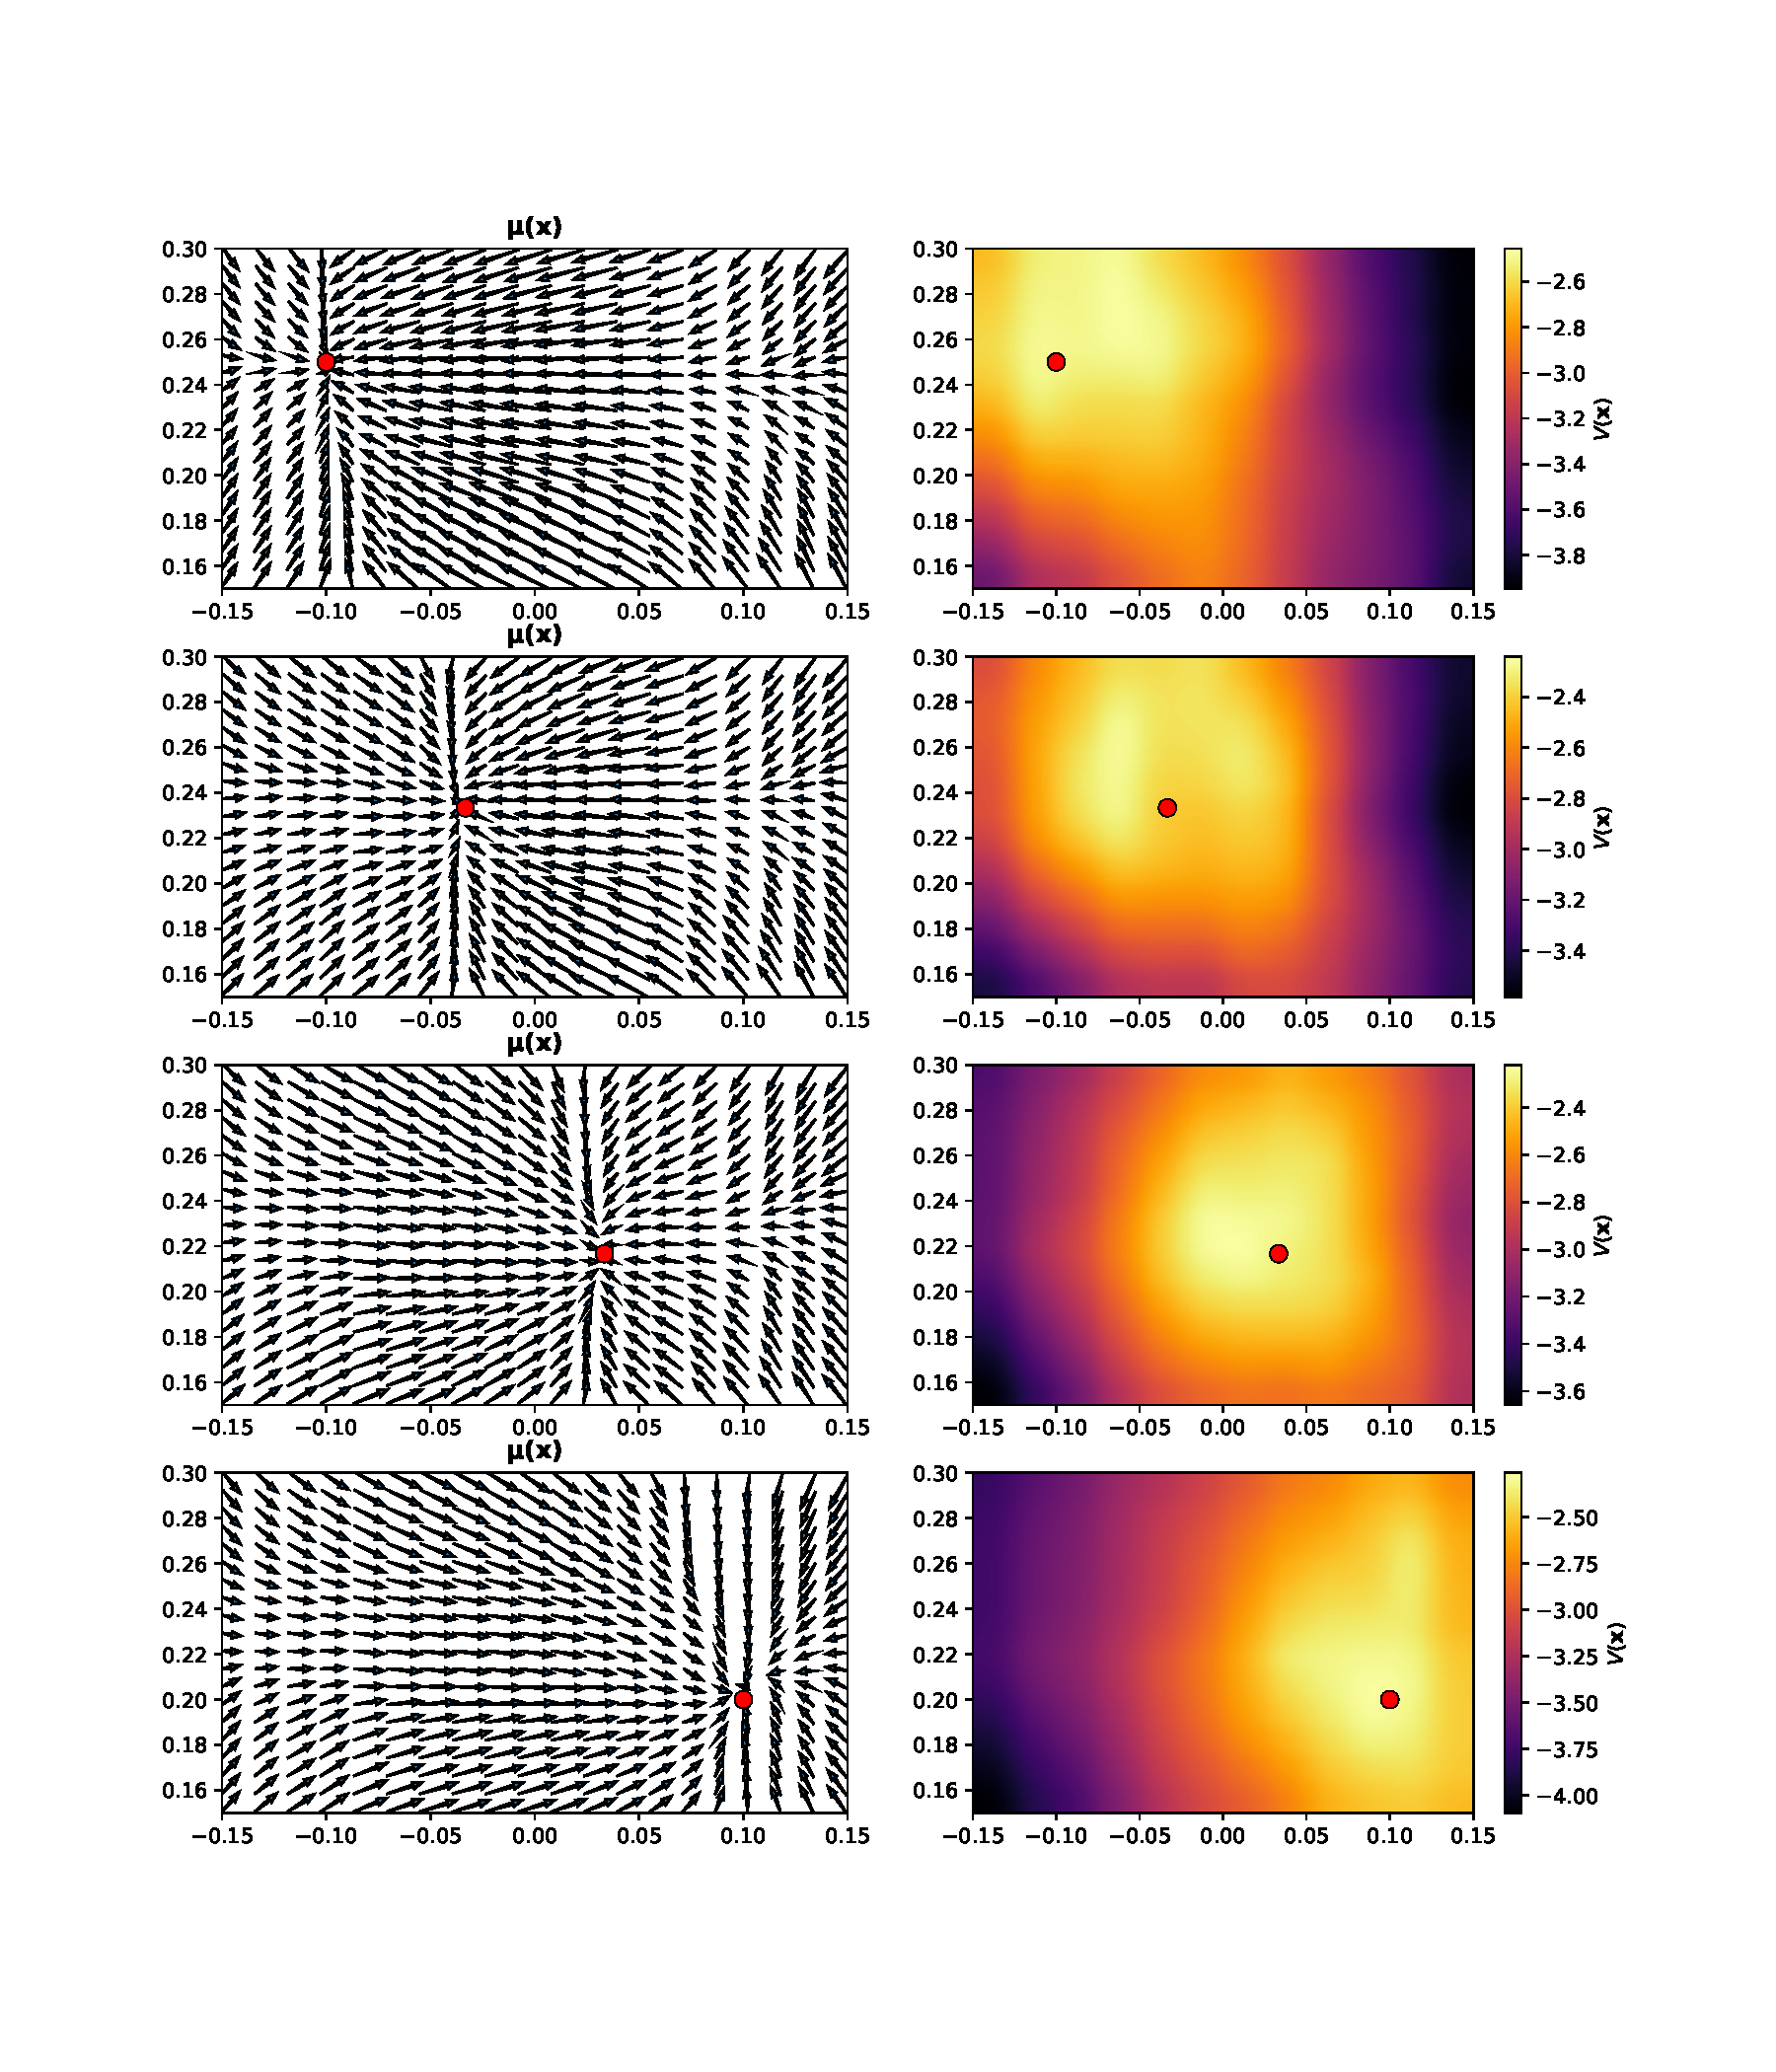
\includegraphics[width=\textwidth]{res/moving_goal_summary.pdf}

    \caption{Trained policy and value function for moving a simulated
    end-effector to randomly set goals. Vertical and horizontal axes are
    end-effector positions. Red dot is goal position. Left figure shows the
    learned policy $\mu$, right side shows the learned value function for
    different goal poses.}

    \label{fig:sim_moving_goal}
    
\end{figure}

\section{Exp2: Robot reaching}

To investigate whether the previous simulated experiment would generalize to
real robotic arms, robots were set up to do a reaching task, where a central
server maintained a replay buffer, parameters, and executed training. Data
collection was distributed over three robots with respective computers.

\subsection{Algorithms and Equipment}

The same setup as in the previous experiment was used with the distributed
version of NAF. The policy was trained on a separate server equipped with a
GPU. Three low-cost robotic arms with three degrees of freedom were used where
different poses were achieved by setting angles of the three servos. A
controller and kinematics were implemented and derived in order to measure and
command poses of the end-effector in cartesian space. For every arm, there was
one dedicated computer, local workers, that evaluated the latest policy given
the arm pose and sent the transitions to the server. The robot with the
coordinate frame is shown in figure \ref{fig:uarm_coordinate_frame} a) and the
entire setup (excluding server) is shown in \ref{fig:uarm_coordinate_frame} b).

\begin{figure}[ht]
    \centering
    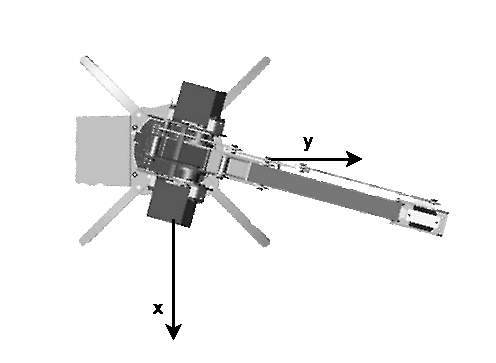
\includegraphics[width=0.39 \textwidth]{res/uarm_coordinates.pdf}
    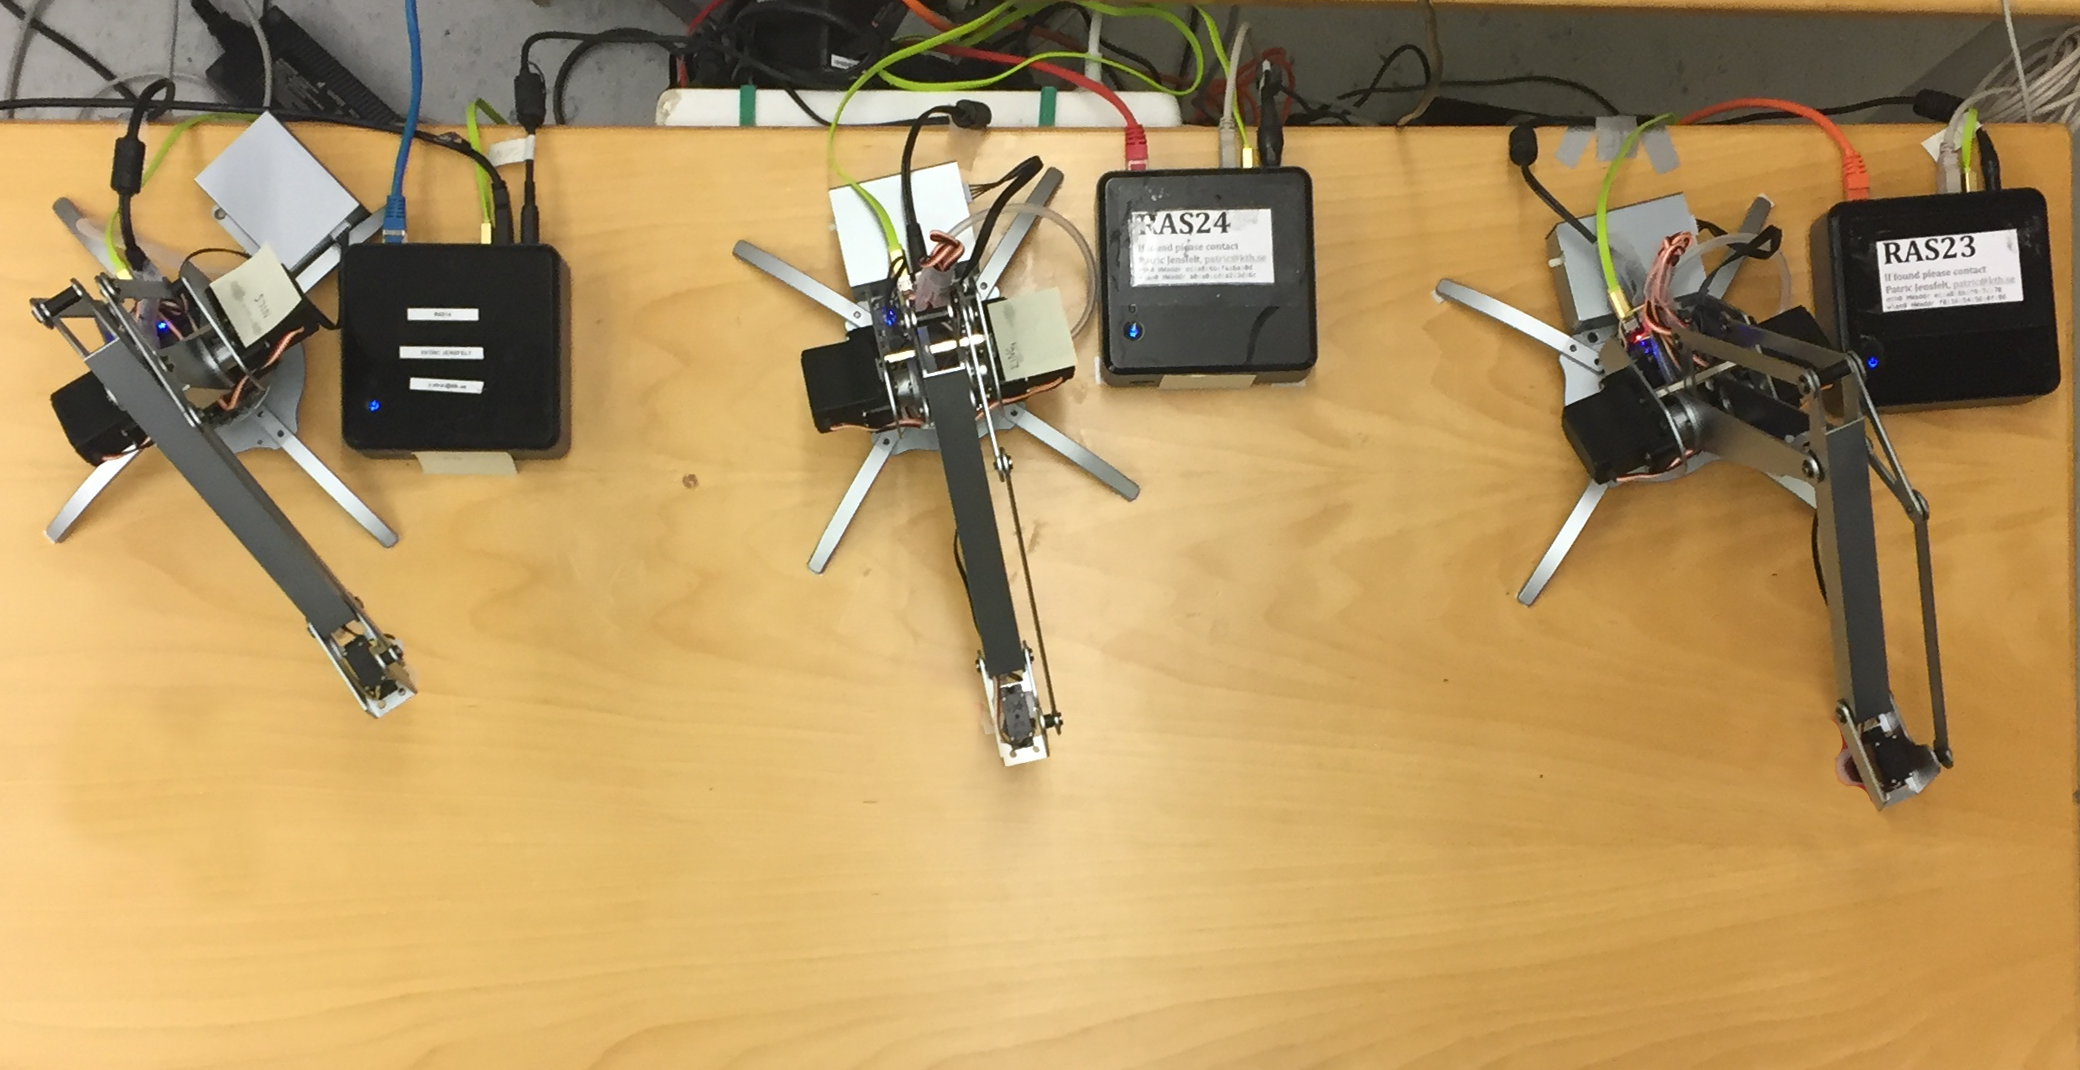
\includegraphics[width=0.59 \textwidth]{res/uarm_moving_setup.png}

    \caption{a) Coordinate frame used. b) The setup of the robot arms along
    with their dedicated computers.}

    \label{fig:uarm_coordinate_frame}
    
\end{figure}

In order to facilitate communication of recorded state transitions and fetching
updated parameters, a server was implemented enabling PUT and GET requests from
the local workers.

\subsection{Data gathering}

Before and after each action was sent to the robot arm, poses of the arm were
measured. This process could only be done at approx. $2-4$ Hz, not including
arm re-positioning, making re-runs from scratch time consuming. Therefore, data
gathering was first run on the three robots for $4$ hours without policy
updates, resulting in approximately $80k$ state transitions. The actions were
randomly drawn from $\mathcal{N}(\mathbf{0}, 0.005^2 \mathbf{I})$, and when the
robot arm reached outside the workspace, or reached within $1$ cm of the
target, the end-effector was replaced at a new random starting position. The
commands were 2-dimensional vectors representing the relative movement in $x$
and $y$ direction respectively. The $z$-coordinate was kept fixed during the
experiment. When training of the parameters was started on the server, the
robots kept collecting and pushing data to the server, and synchronized
parameters before each reset of the end-effector position. During this phase,
noise was added to the policy during every 3 out of 4 runs, while every 1 out 4
runs the policy was evaluated without noise in order to track progress.

\subsection{Results}

The performance of the policy was evaluated by measuring the average distance
to the target position on the last state before every reset. The progress of
this metric is shown in figure \ref{fig:uarm_moving_goal_progress}, here shown
with a running mean of width $128$. The trained policy and value function are
shown in figure \ref{fig:uarm_moving_goal_policy}.

\begin{figure}[h!]
    \centering
    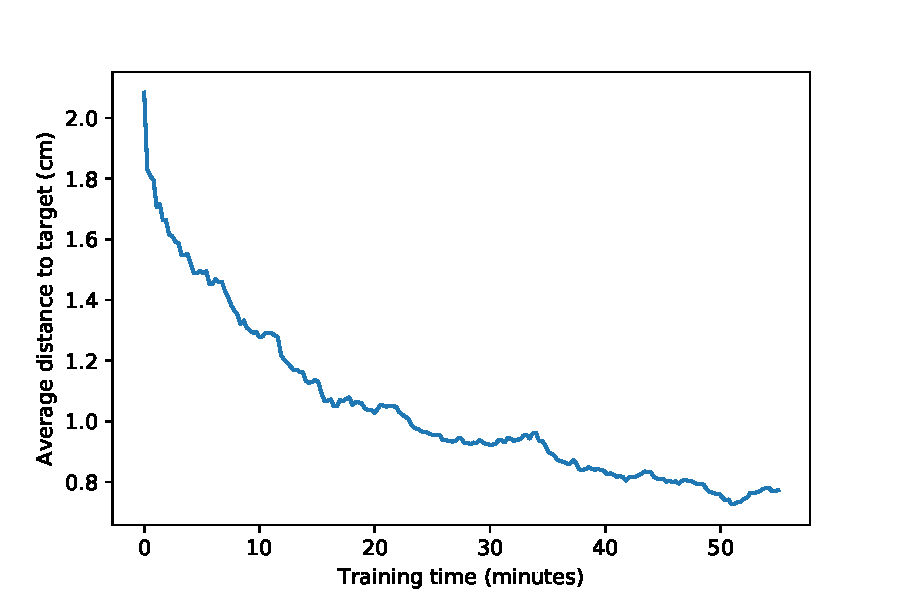
\includegraphics[width=0.50 \textwidth]{res/uarm_moving_goal_progress.pdf}

    \caption{Average final distance to target pose.}
    \label{fig:uarm_moving_goal_progress}
    
\end{figure}

\begin{figure}[h]
    \centering
    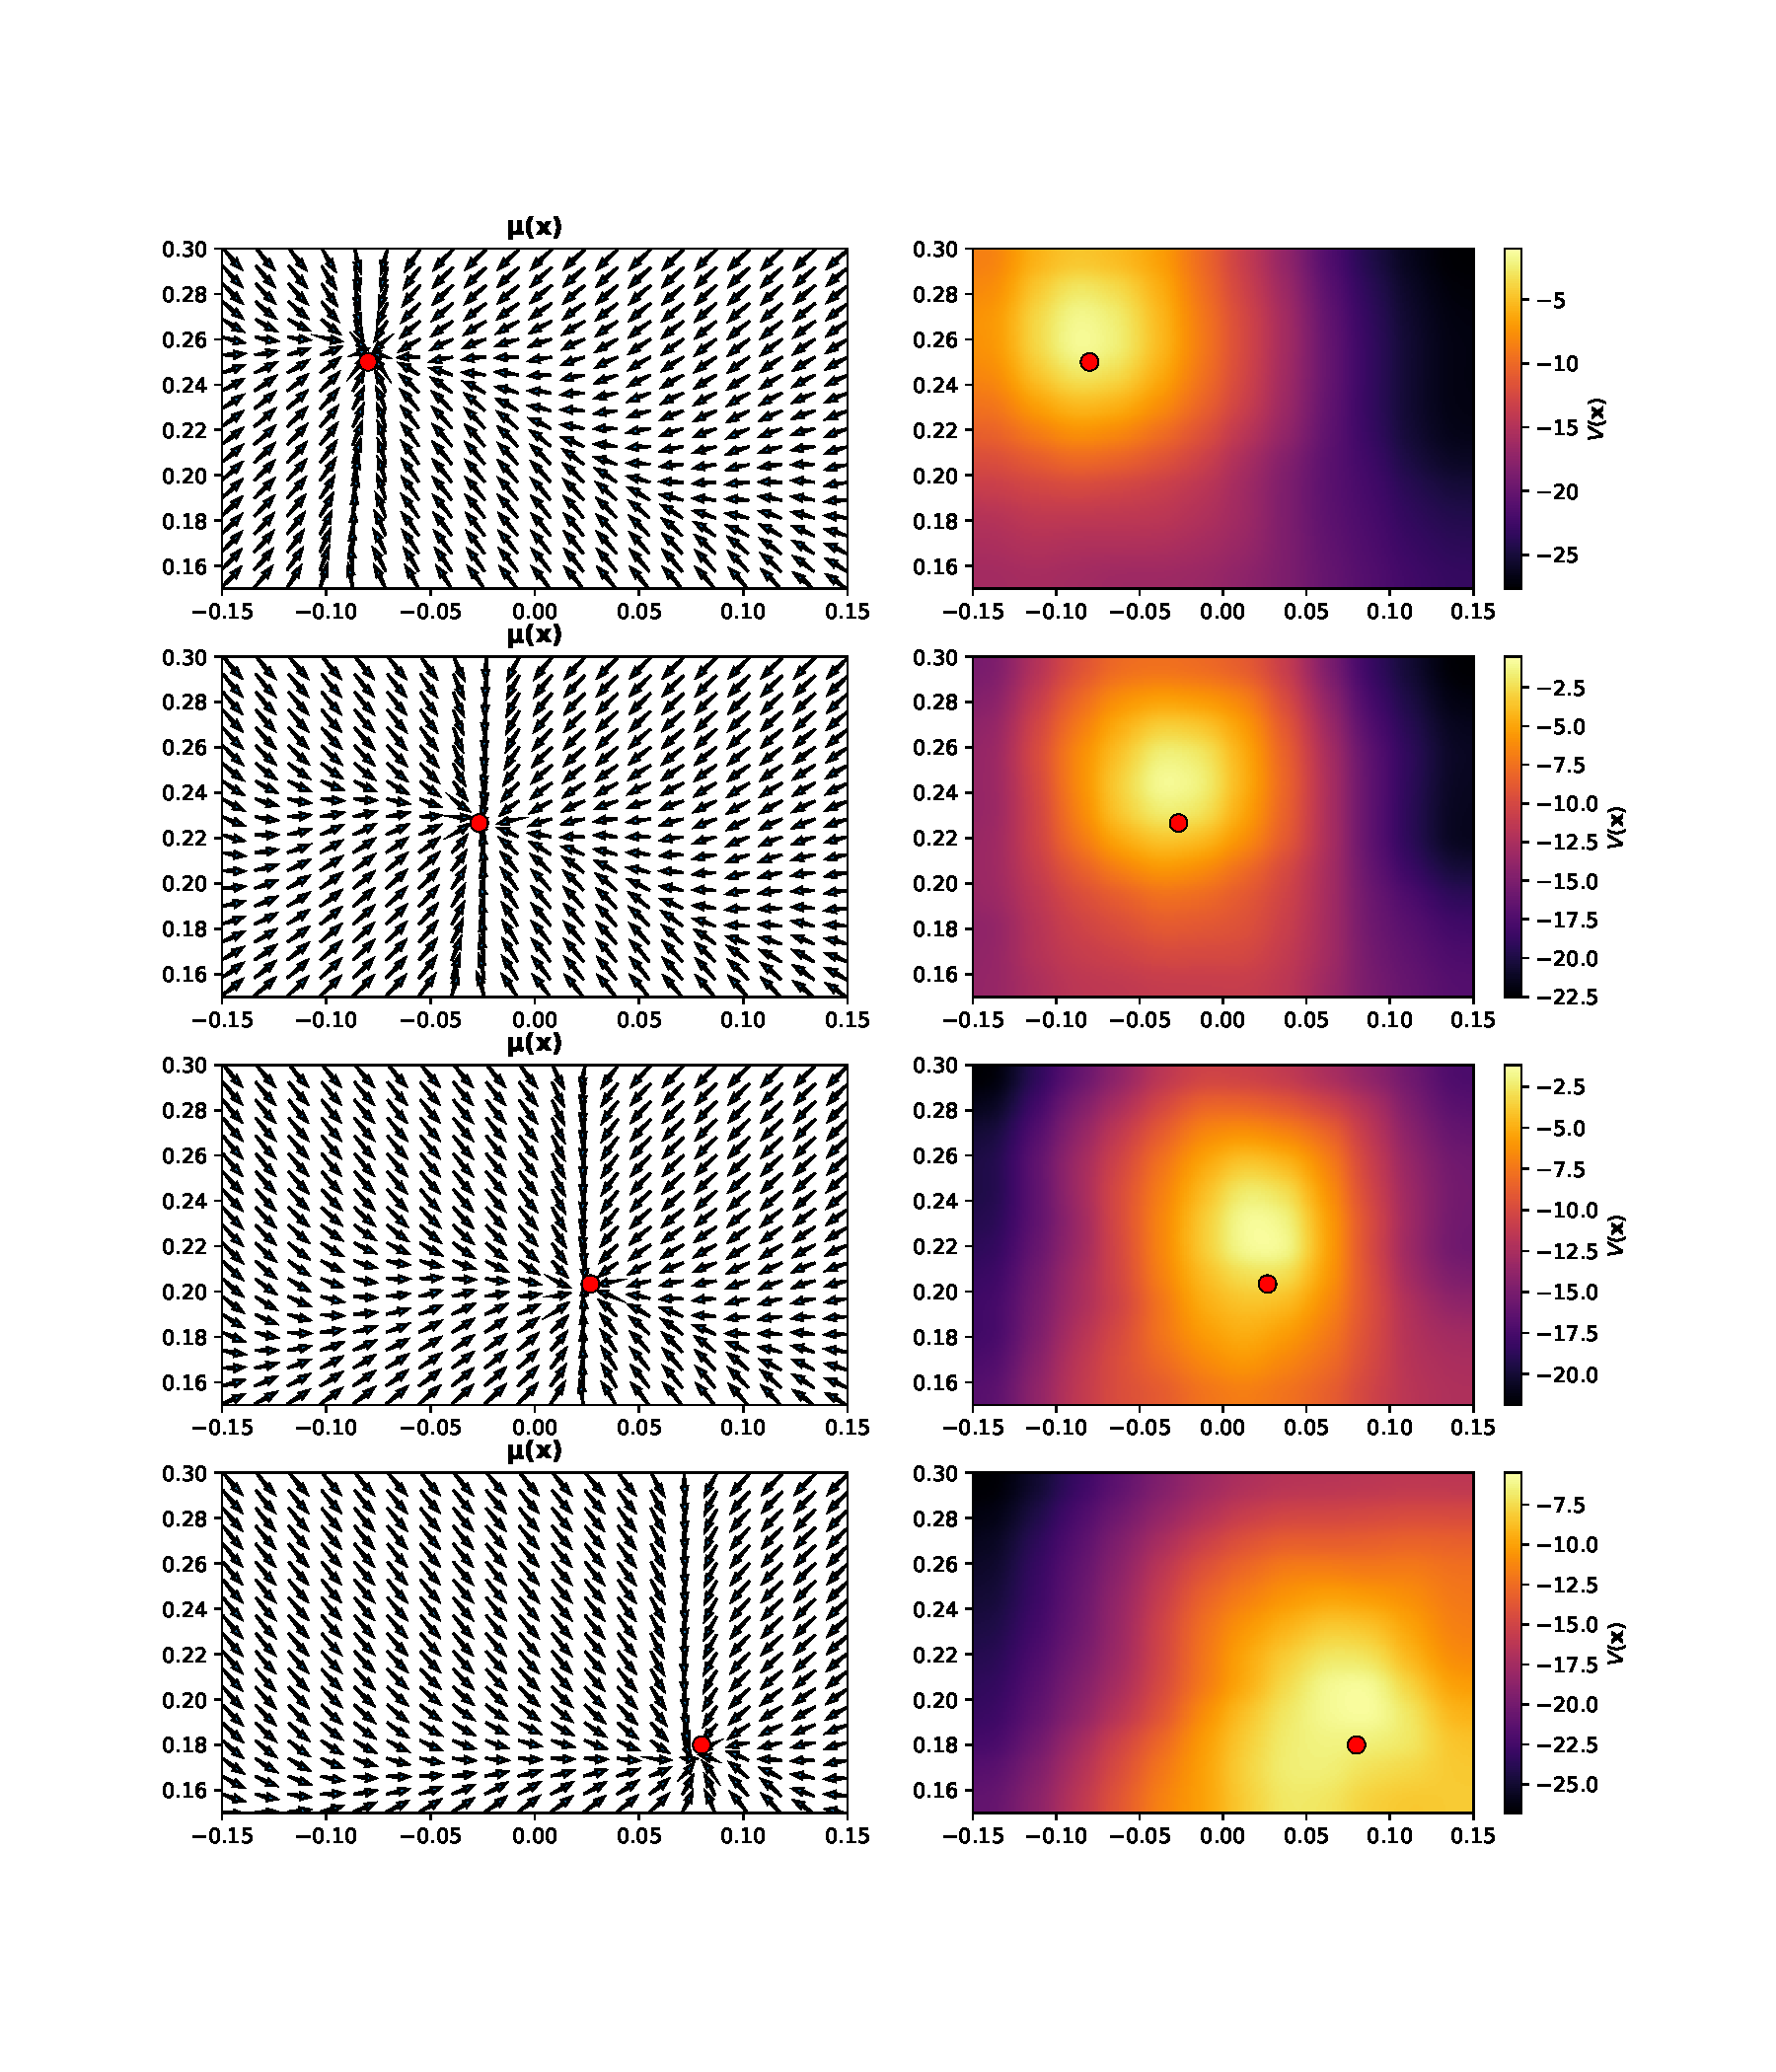
\includegraphics[width=\textwidth]{res/multiple_goals_uarm.pdf}

    \caption{Robot multiple goal poses of EEF}
    \label{fig:uarm_moving_goal_policy}
    
\end{figure}

%\begin{figure}[h]
%    \centering
%    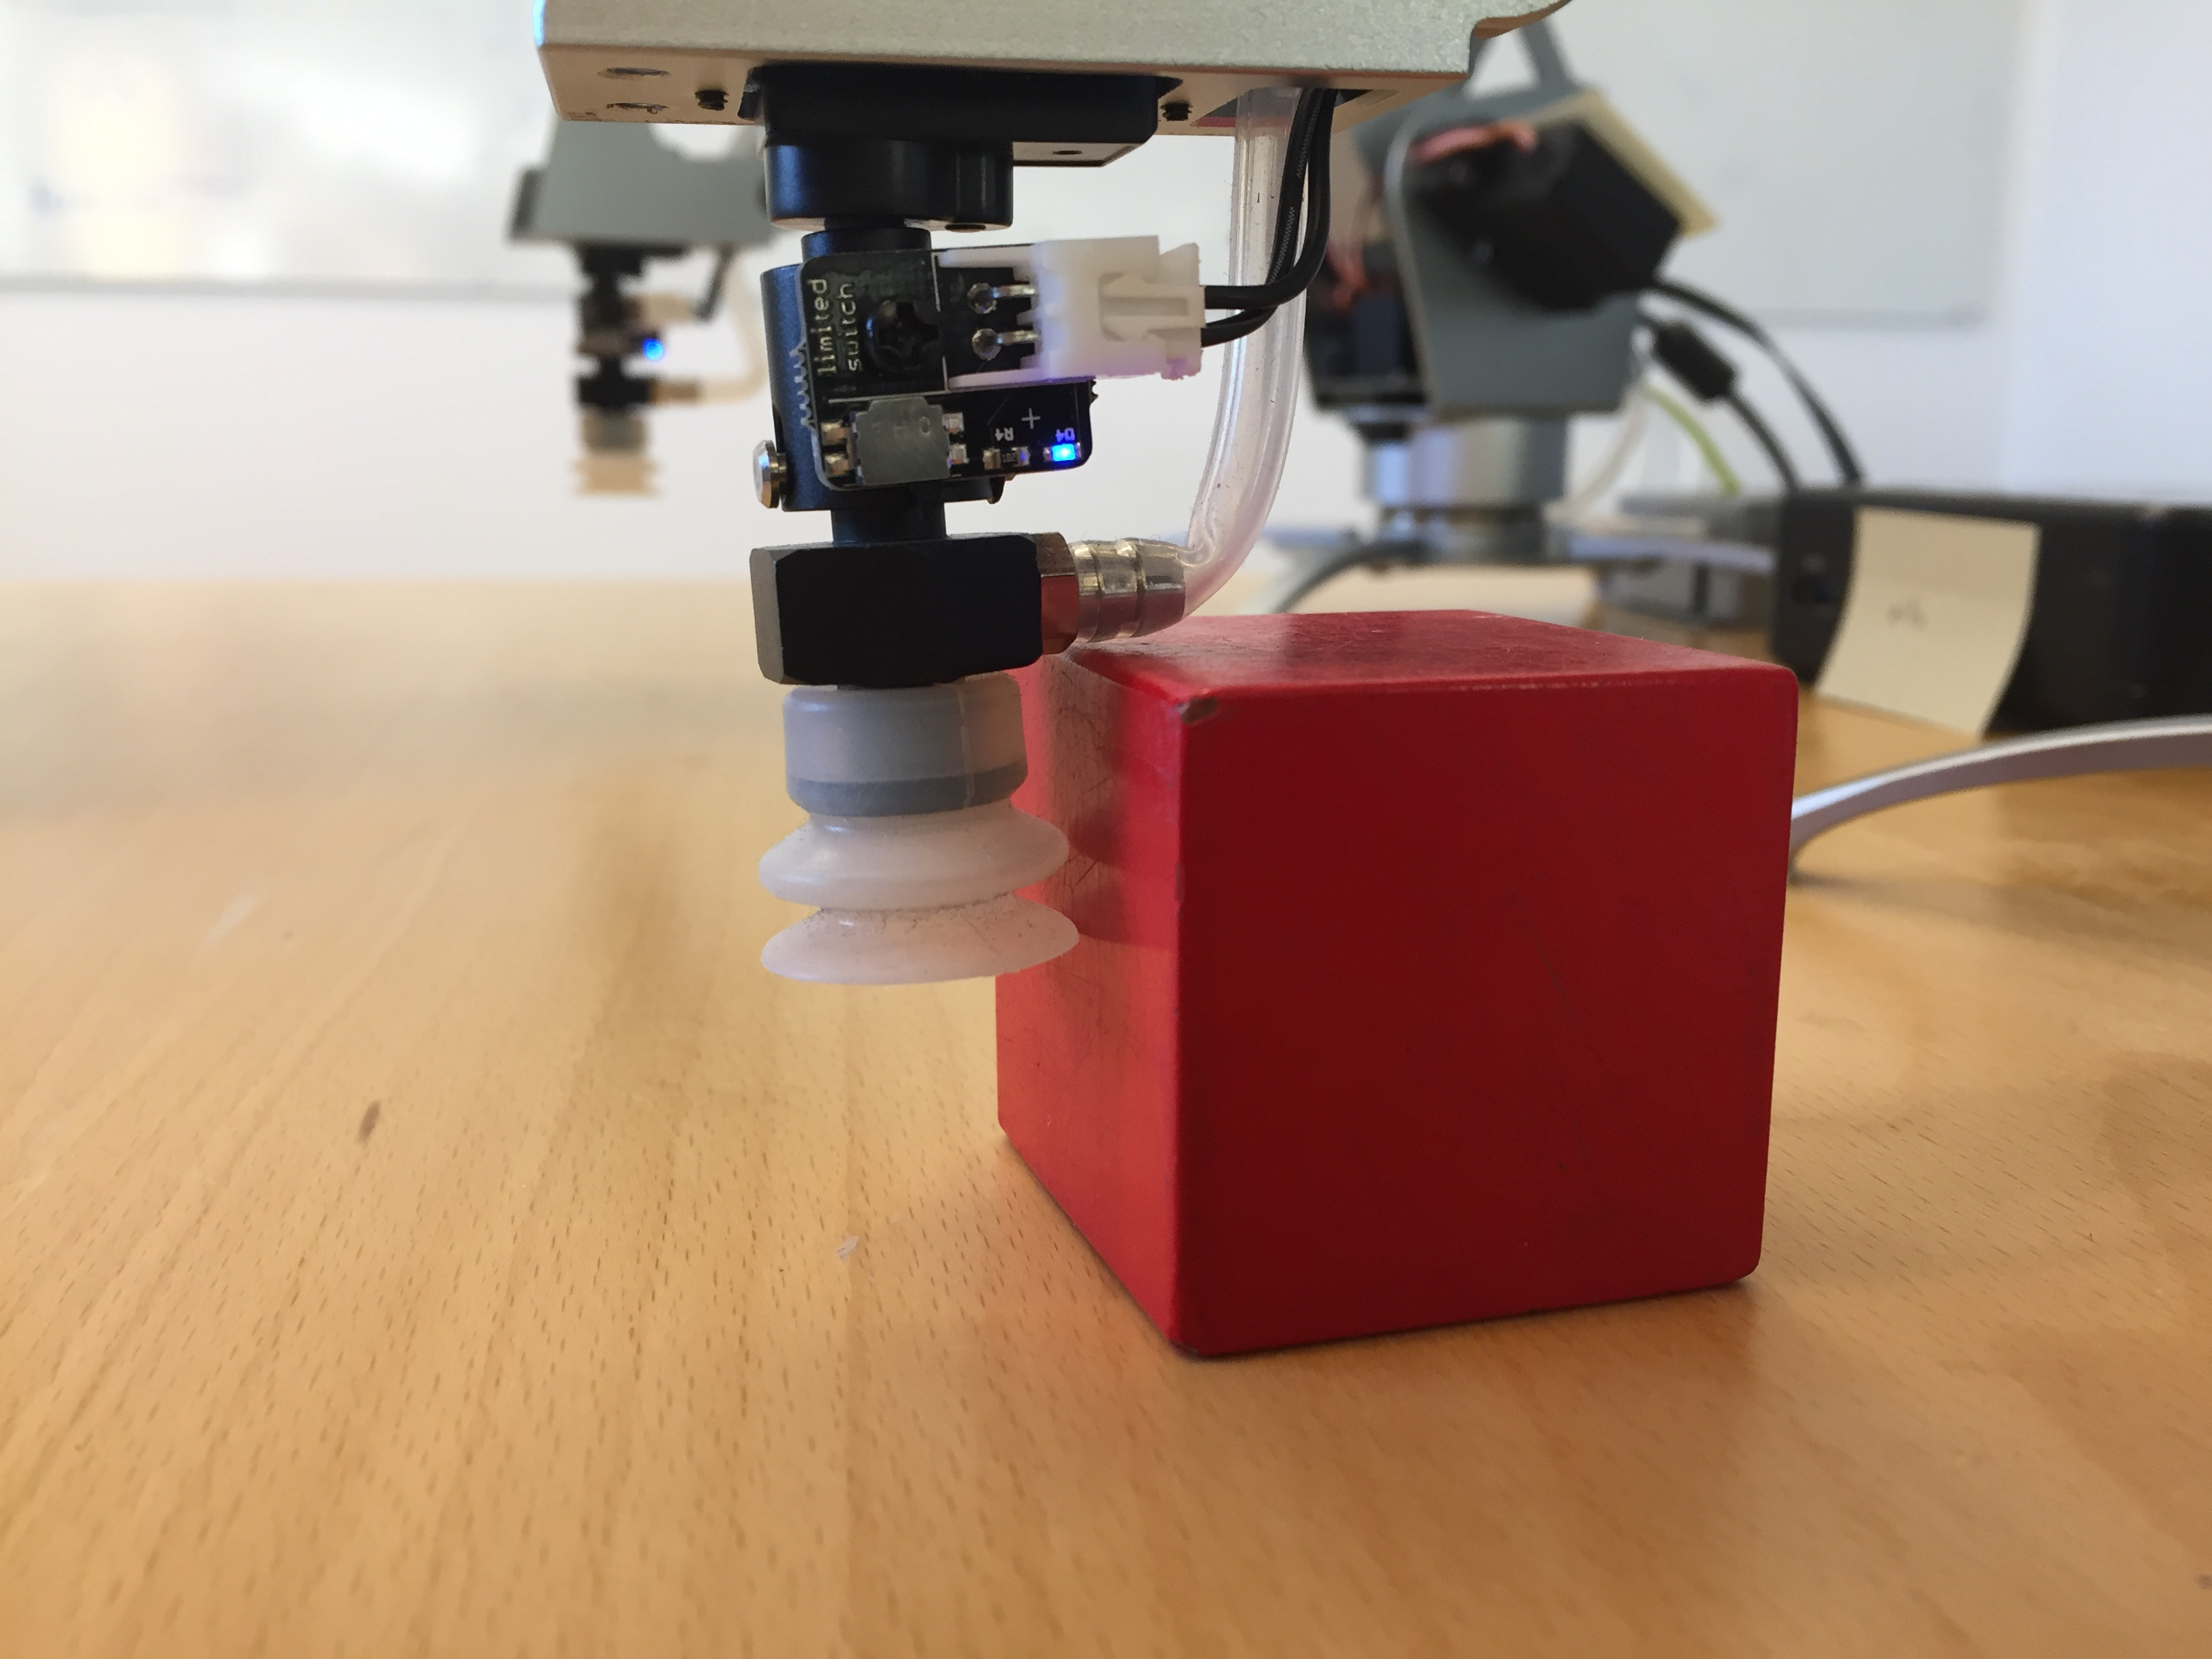
\includegraphics[width=0.40 \textwidth]{res/eef_cube_low.jpg}
%    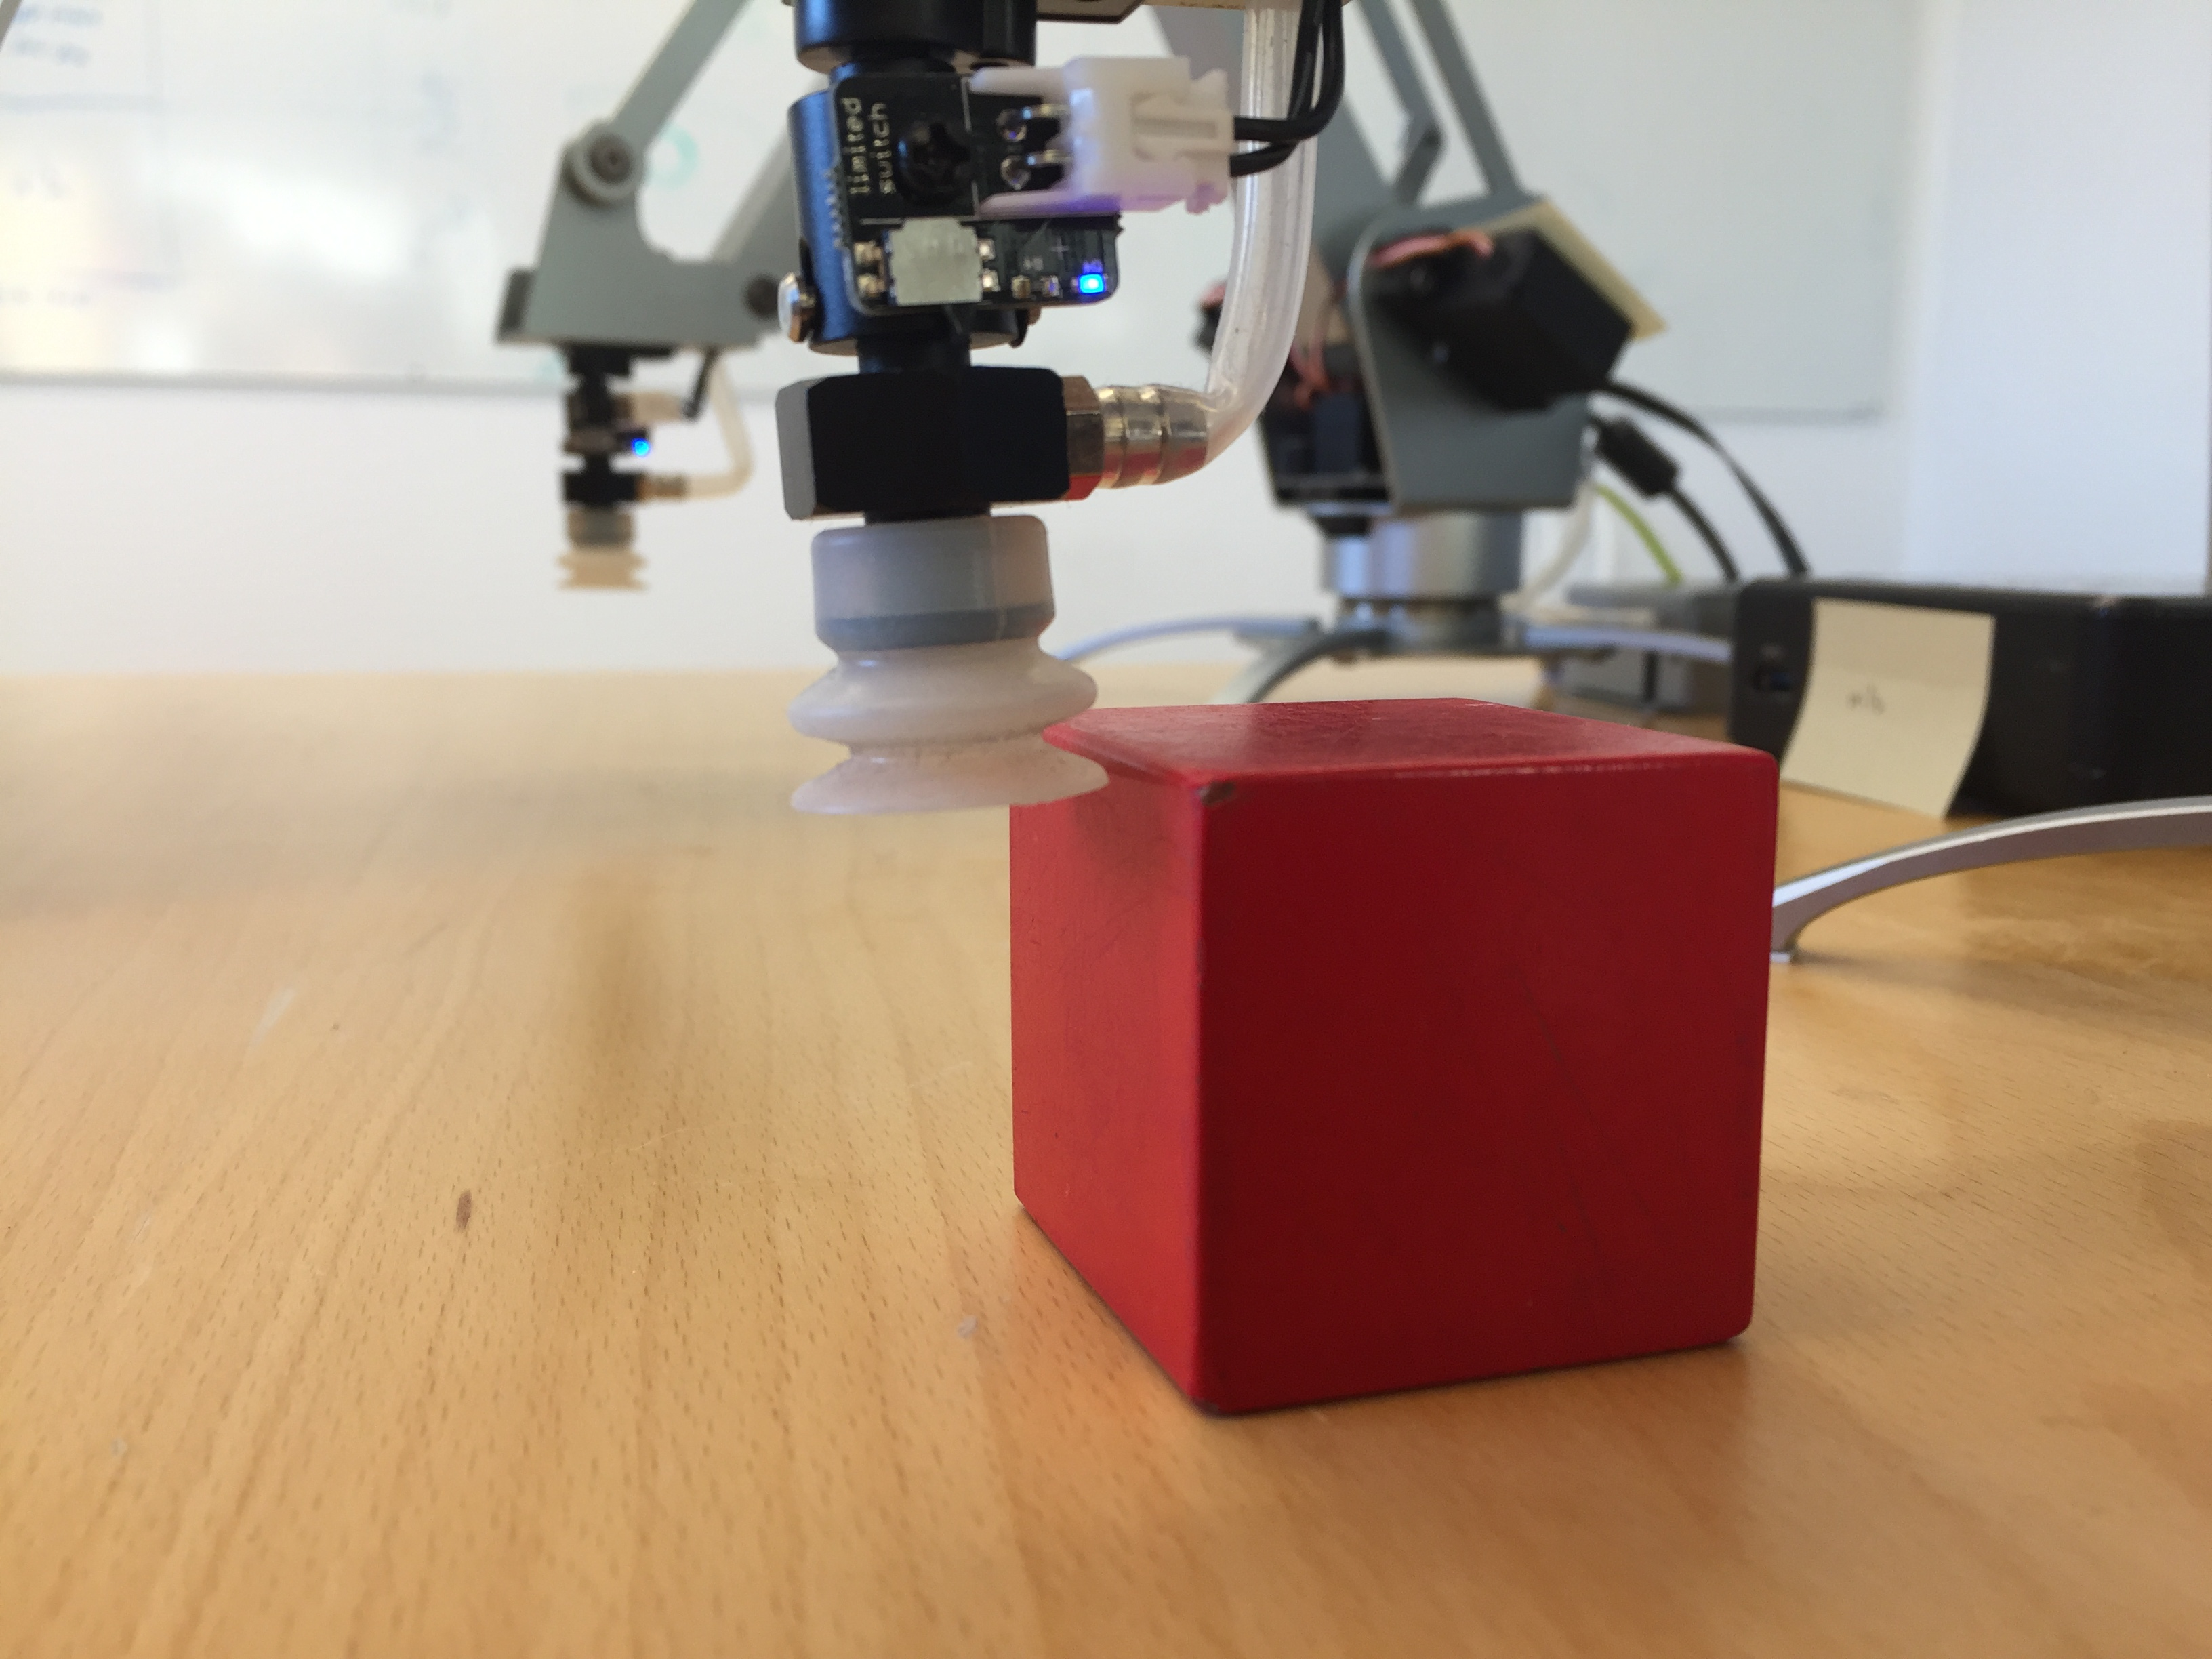
\includegraphics[width=0.40 \textwidth]{res/eef_cube_high.jpg}
%
%    \caption{Possible $z$-values of the eef. TODO: Finish/polish this}
%    
%\end{figure}

\section{Exp3: Pushing task in simulation}
The next task was to push a square cube into some target position using
the real robot arm, however preliminary experiments using NAF did not
converge to an intuitively good policy. Instead of rejecting the capabilities
of the NAF algorithm at this stage, simulation experiments was first done in
an ideally setup environment.

\subsection{Environment}

\subsection{Algorithms}

\subsection{Results}

\begin{figure}[h!]
    \centering
    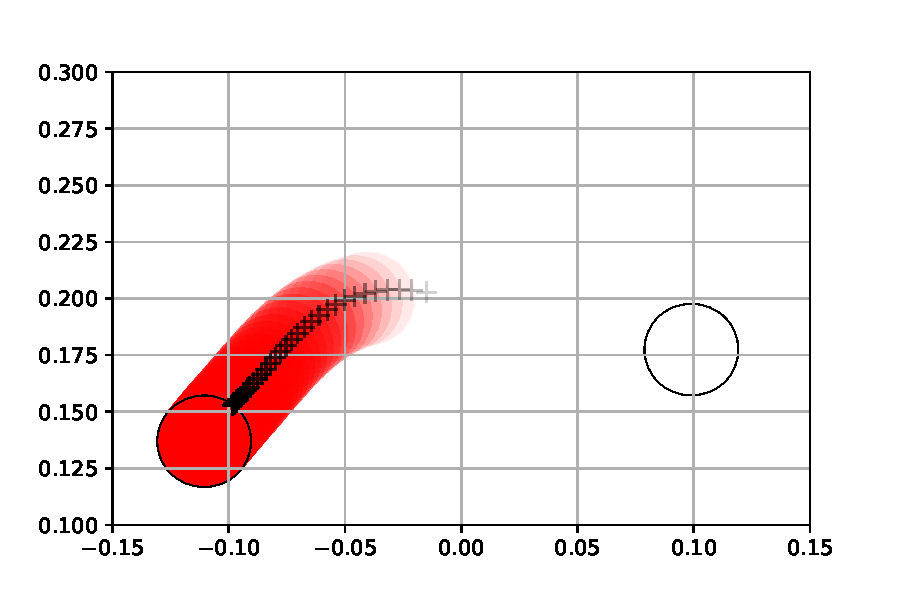
\includegraphics[width=0.4 \textwidth]{res/naf_sim_failure_mode.pdf}
    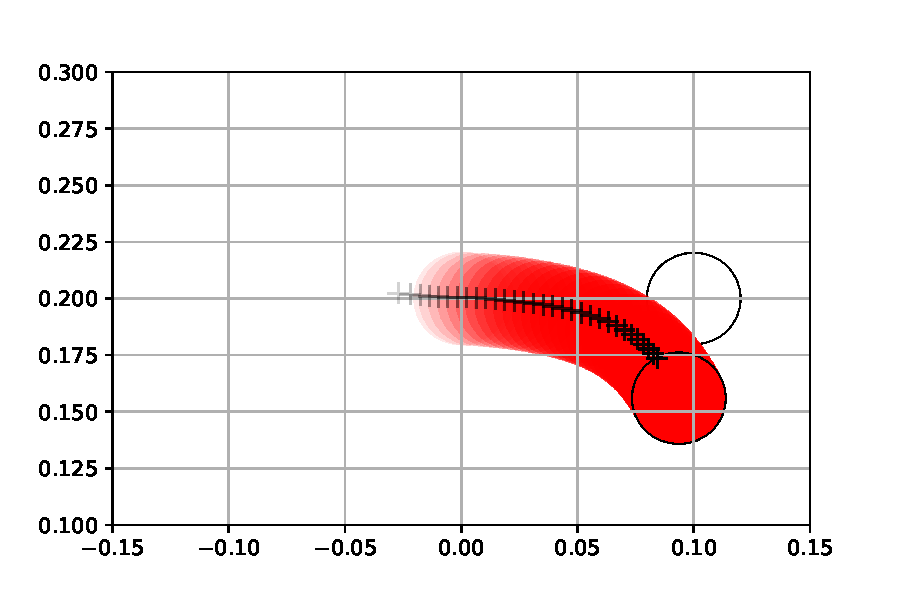
\includegraphics[width=0.4 \textwidth]{res/naf_sim_failure_mode_ideal.pdf}

    \caption{Results of NAF in simulation on pushing task. The red circle is
    the object being pushed, the white circle is the goal, and the cross is the
    simulated end-effector.}

    \label{fig:naf_sim_failure}
\end{figure}

\begin{figure}[h!]
    \centering
    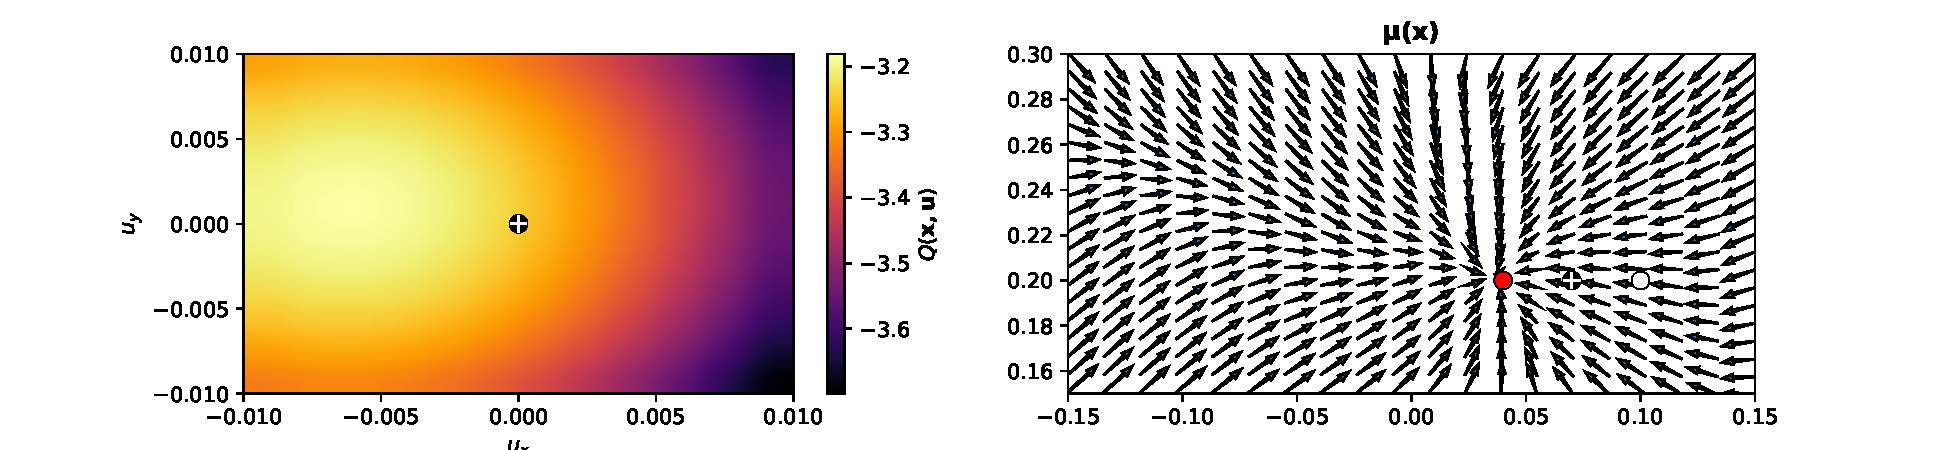
\includegraphics[width=1.0 \textwidth]{res/naf_sim_unimode_q.pdf}

    \caption{Results from using NAF on a simulated pushing task. Q-function and
    policy of the state given by the pushable object (red), the goal (white
    circle), and the end-effector (white cross). Since the advantage function
    is parameterized by a quadratic expression, which is uni-modal, the
    Q-function cannot place more mass on actions corresponding to going up and
    down rather than some intermediate point, and instead in this case the mean
    is placed straight to the left.}

    \label{fig:naf_sim_unimode_q}
\end{figure}

\section{Exp4: Pushing task with pose estimation from LIDAR}

This aim of this experiment was to show that a policy could be learned on
real robots for pushing a cube to some target pose.

\subsection{Equipment}

To measure the poses of the cubes, a \textit{LIght Detection And Range} (LIDAR)
was used by placing it in front of the robot arm (left side of figure
\ref{fig:eef-frame}) TODO. The poses of the cubes was given in the end-effector
frame shown to the right in figure TODO \ref{fig:eef-frame}. The transformation from
LIDAR-frame to robot-frame was found by sampling robot-frame poses and using a
least-squares approach rather than explicitly measuring translation and
rotation. The poses of the cubes consisted of the $x$ and $y$ coordinates of the
center of the cube and the rotation only given in the first quadrant due to
symmetries. The rotation was although ignored due to low precision, only
keeping the $x$ and $y$ position.

\begin{figure}[h!]
    \centering
    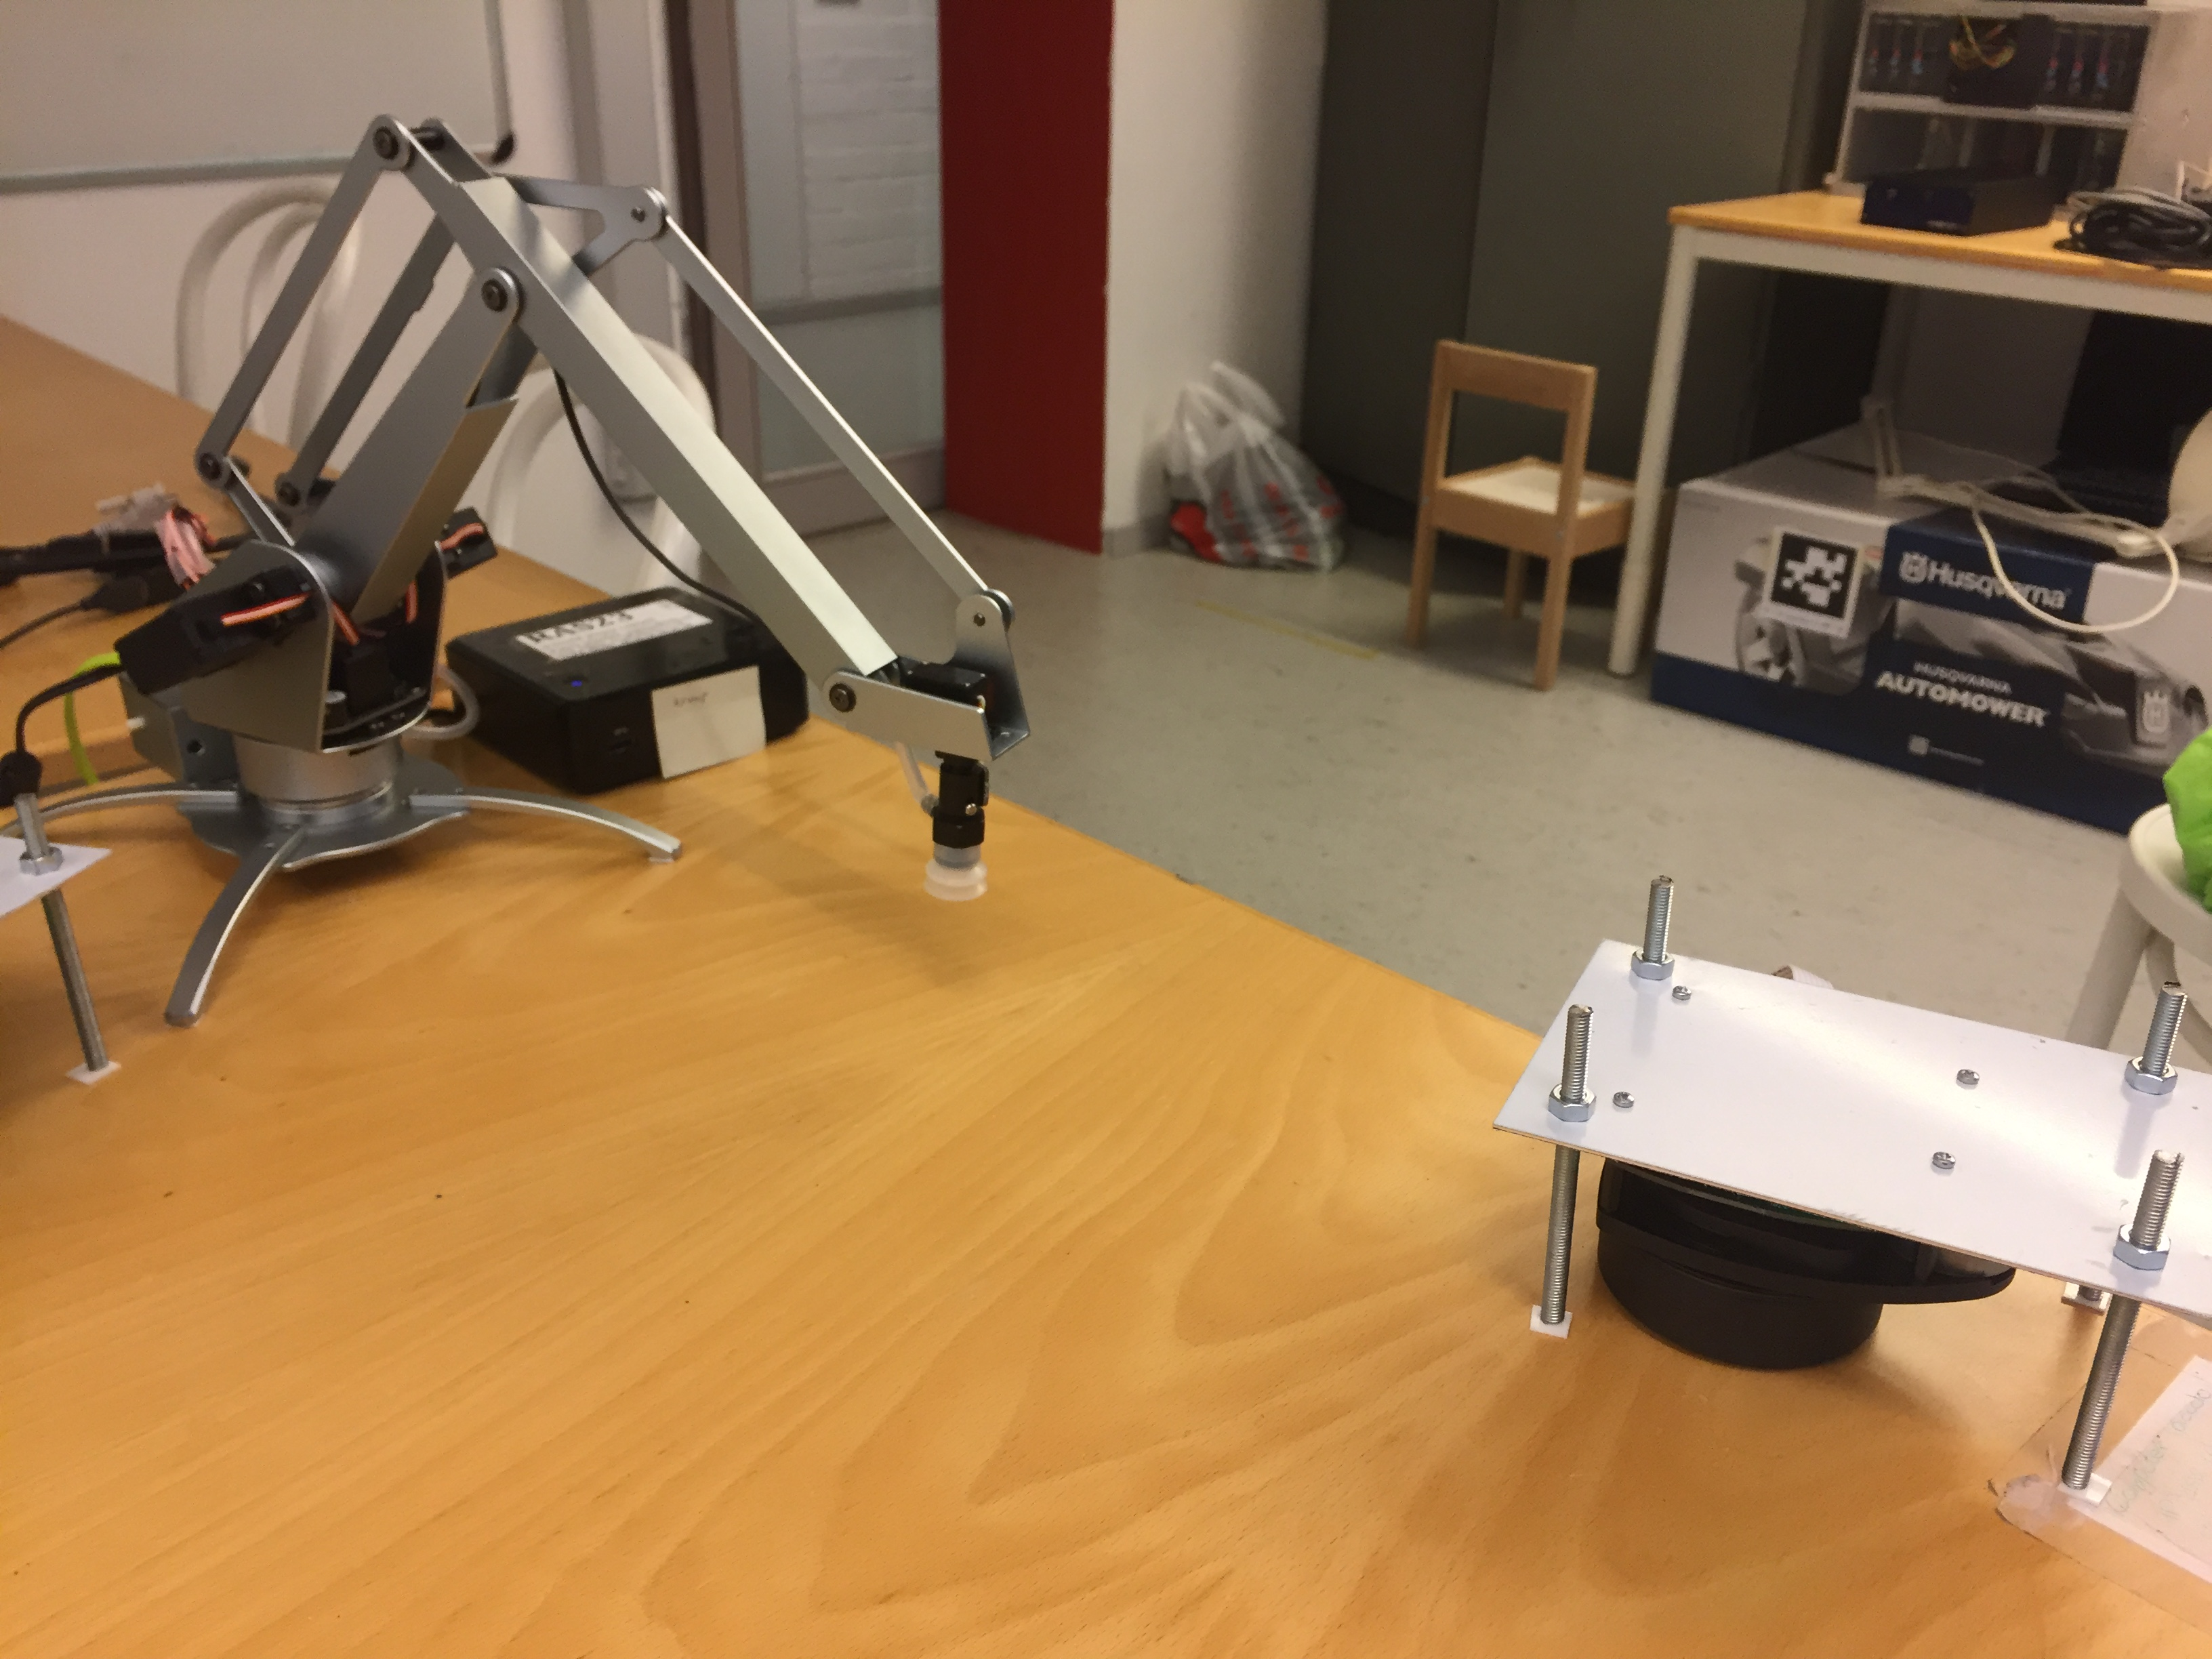
\includegraphics[width=0.48 \textwidth]{res/lidar_placement.JPG}

    \caption{TODO}
    \label{fig:eef-frame}
    
\end{figure}

\section{Exp5: Pushing task with pose estimation from LIDAR}

This aim of this experiment was originally to show that a policy could be
learned on real robots for pushing a cube to some target pose. However,
experiments in simulation were harder than anticipated and consumed several
weeks before solving the problem. Also, when adding the same amount of noise
expected to come from sensors to the simulation problem, it failed to converge
to any decent policy. The policy trained in the non-noisy simulation worked
quite well when applied to the real setup which is described in more detail
below.

\subsection{Pose estimation}

To estimate the pose of the cube, a \textit{LIght Detection And Range} (LIDAR)
was used by placing it in front of the robot arm (figure \ref{fig:eef-frame}).
The LIDAR returns $360$ distance measurements at approximately evenly spaced
angles which vary from scan to scan. One series of scans is returned at $10$
Hz. The cube is a red wooden cube with all sides measuring $4$ cm. One of these
sides can be found from the LIDAR-measurements by plotting the points onto a
matrix/image and using the Hough transform \cite{duda1972use}. The Hough
transform returns the equations for the lines that make up the sides of the
cube, but not where the sides start and end. Once the lines are known, the
starts and ends can easily be inferred from the scans.  Knowing at least one
side of the cube, the rotation and position of the cube can also be inferred.
For the following experiments, only the position of the cube was kept, ignoring
the rotation. Conversion of the found position of the cube to robot-frame was
done using a least-squares approach after randomly placing the cube at several
positions known from the forward-kinematics of the arm.

\begin{figure}[h!]
    \centering
    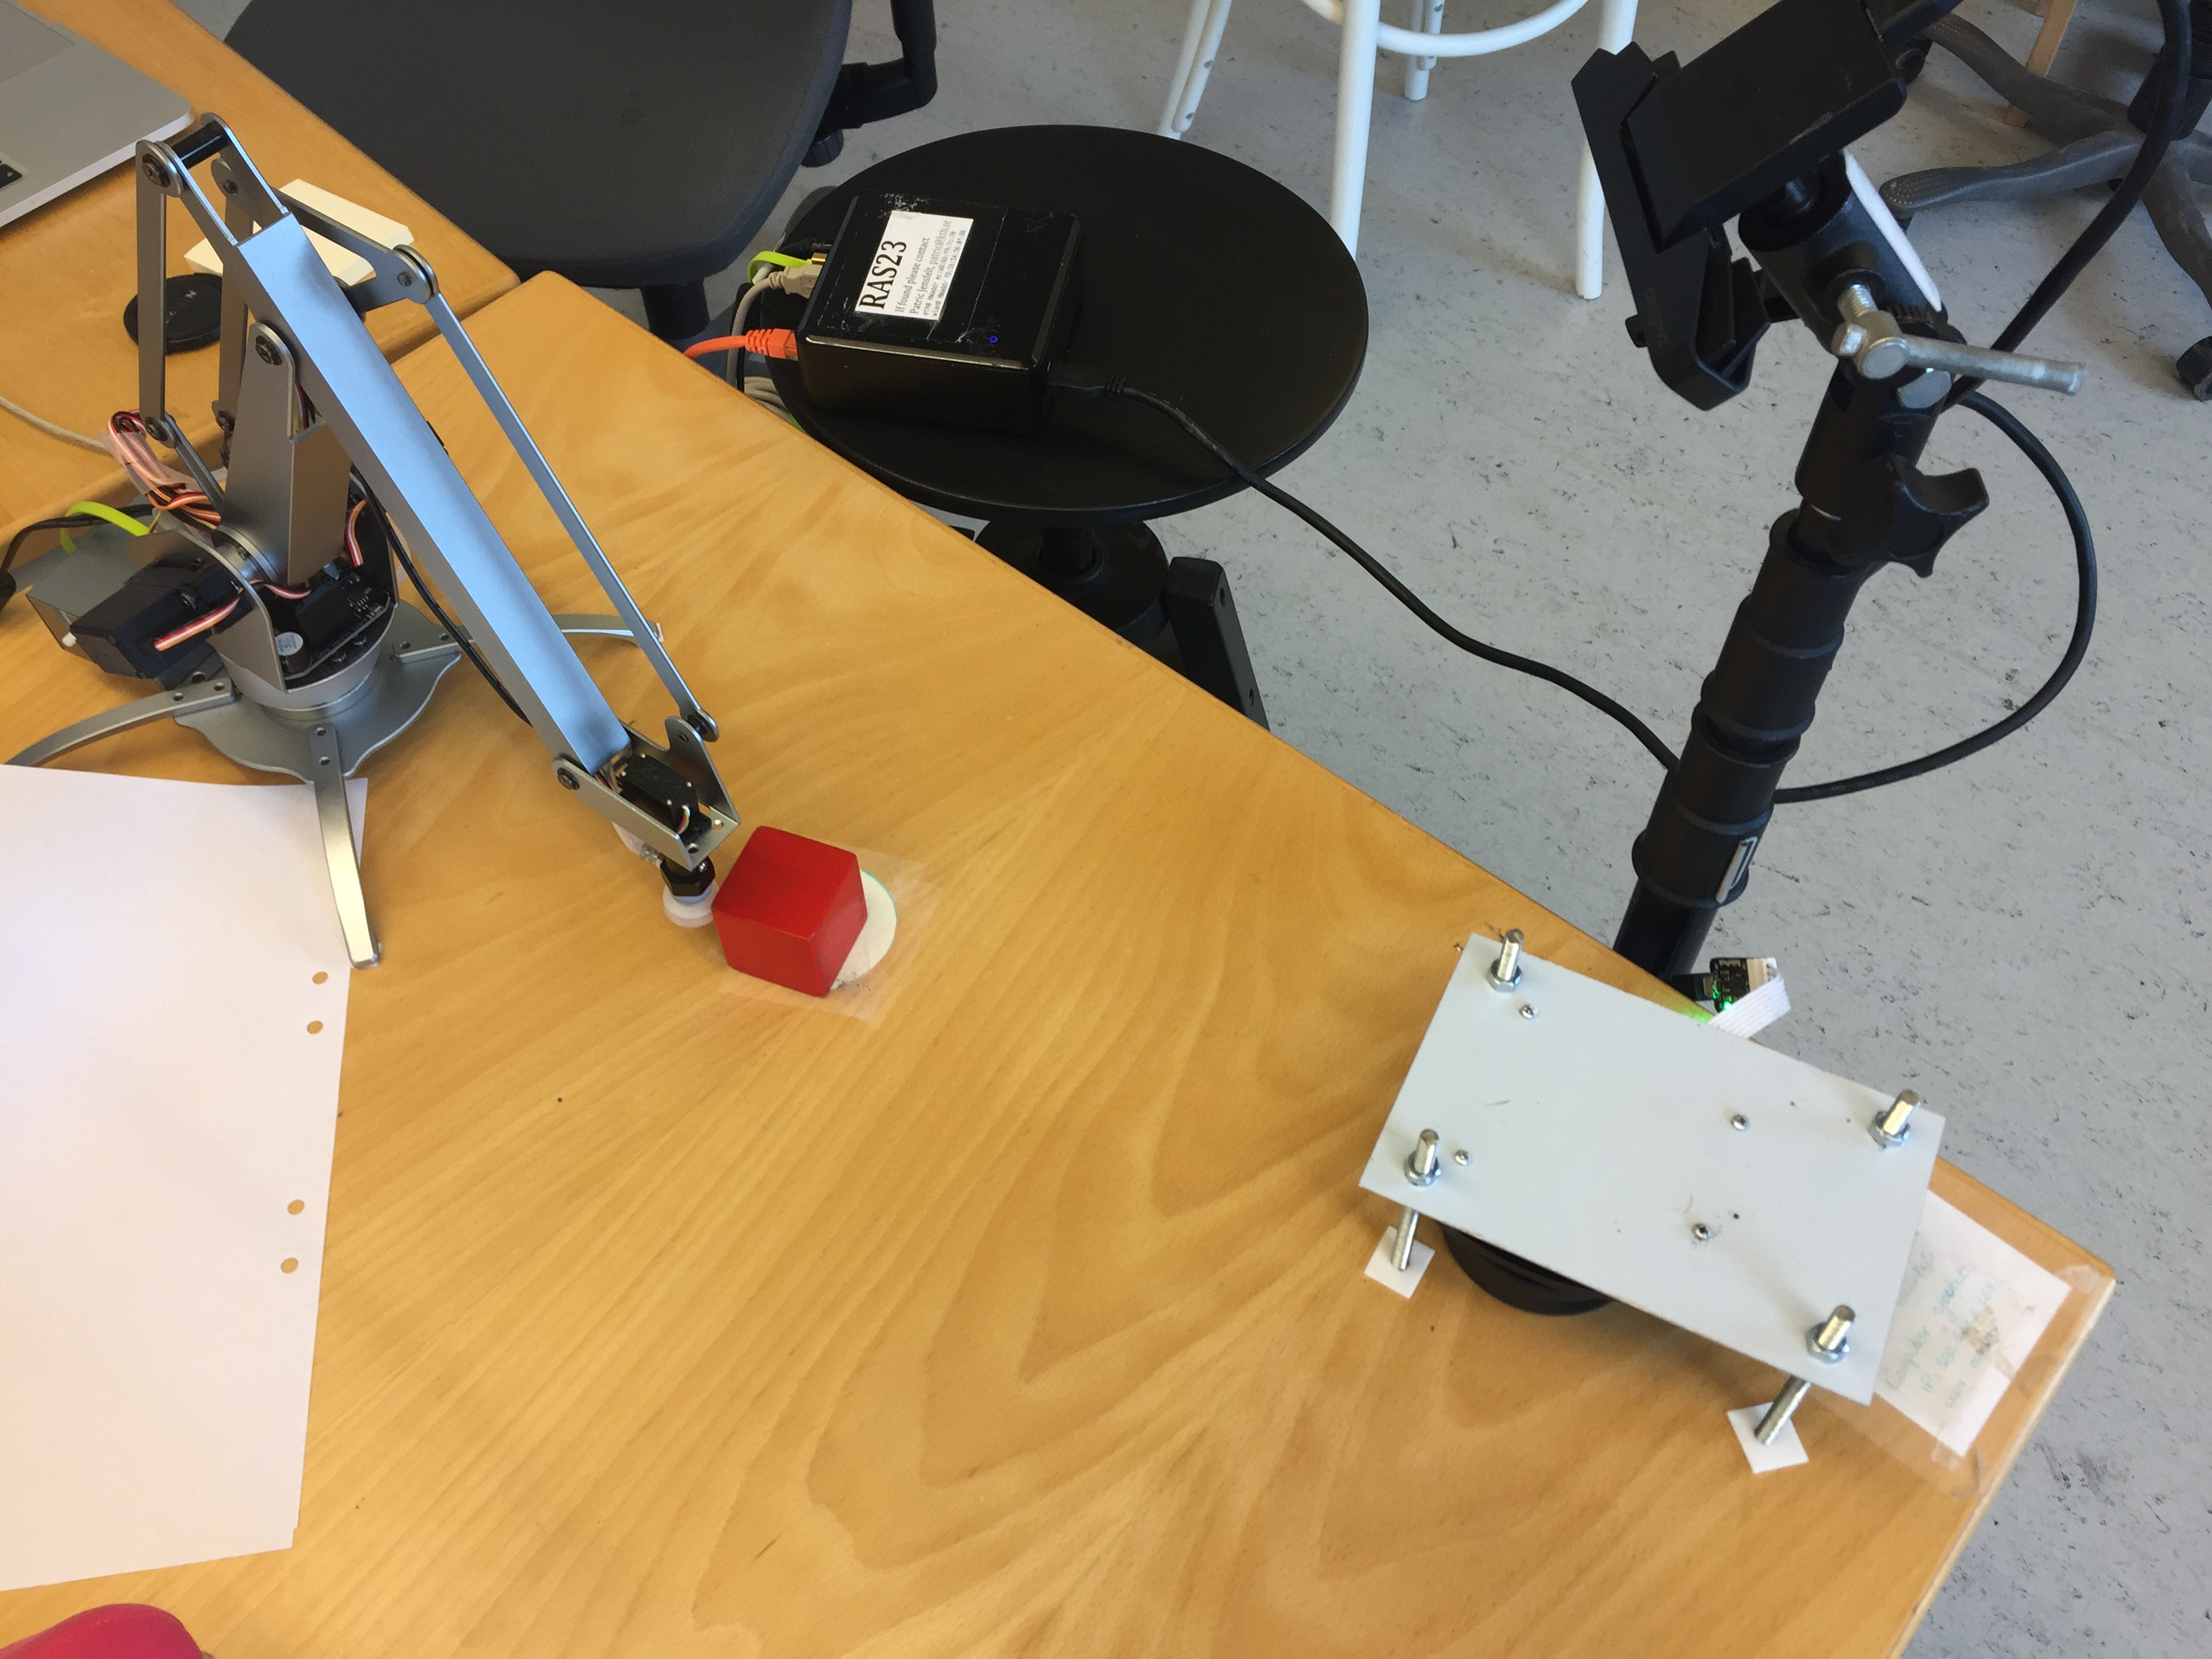
\includegraphics[width=0.48 \textwidth]{res/camera_placement_fixed.jpg}

    \caption{LIDAR seen on the right side in the picture measuring positions of
    the cube. The camera is not used in this experiment.}

    \label{fig:eef-frame}
    
\end{figure}

\subsection{Results}

The policy trained in simulation successfully pushes the cube towards a goal
set in the center of the workspace, video of this can be seen here:
\url{https://youtu.be/82XNDBPbJH0}. Sometimes the policy fails to push the cube
further due to small action commands not affecting the robot, and due to
differences in the shapes of the simulation object (circle) and the cube.
Adding a small noise term alleviated these problems and was used in the linked
video.

\chapter{Pose estimation I: Using a fixed camera}

The policy trained in simulation for pushing a cube to some goal position was
shown to work on the real robotic system with only some minor tweaks.  To know
where the cube was positioned, a LIDAR was used.  Using the LIDAR for pose
estimation of the cube however required that no other objects were accidentally
measured, and used the fact that the position of the cube can be described by a
bounded line in the plane. A more general approach is to infer the pose from a
camera. A usual setup in robotics is to have a camera at a fixed position and
infer poses under the assumption that the camera does not shift position.
Experiments are here first described for estimation under this assumption and
then extended for estimation from a non-fixed camera.

\section{Method}

A camera was mounted at a fixed position as shown in figure
\ref{fig:camera_placement_fixed}. A LIDAR was used to label the pose of the
cube in the coordinate frame of the robot. In total, 10'000 RGB images were
collected during execution of the trained policy. For each picture, depth
channel data was also collected to evaluate the difference in performance when
adding this information. For the depth channel, the camera returns numbers in
the range $[0, 255]$ aligned for each pixel in the color image. The distance
$0$ is in practice never registered but used to represent that depth for this
pixel is missing.

\begin{figure}[h!]
    \centering
    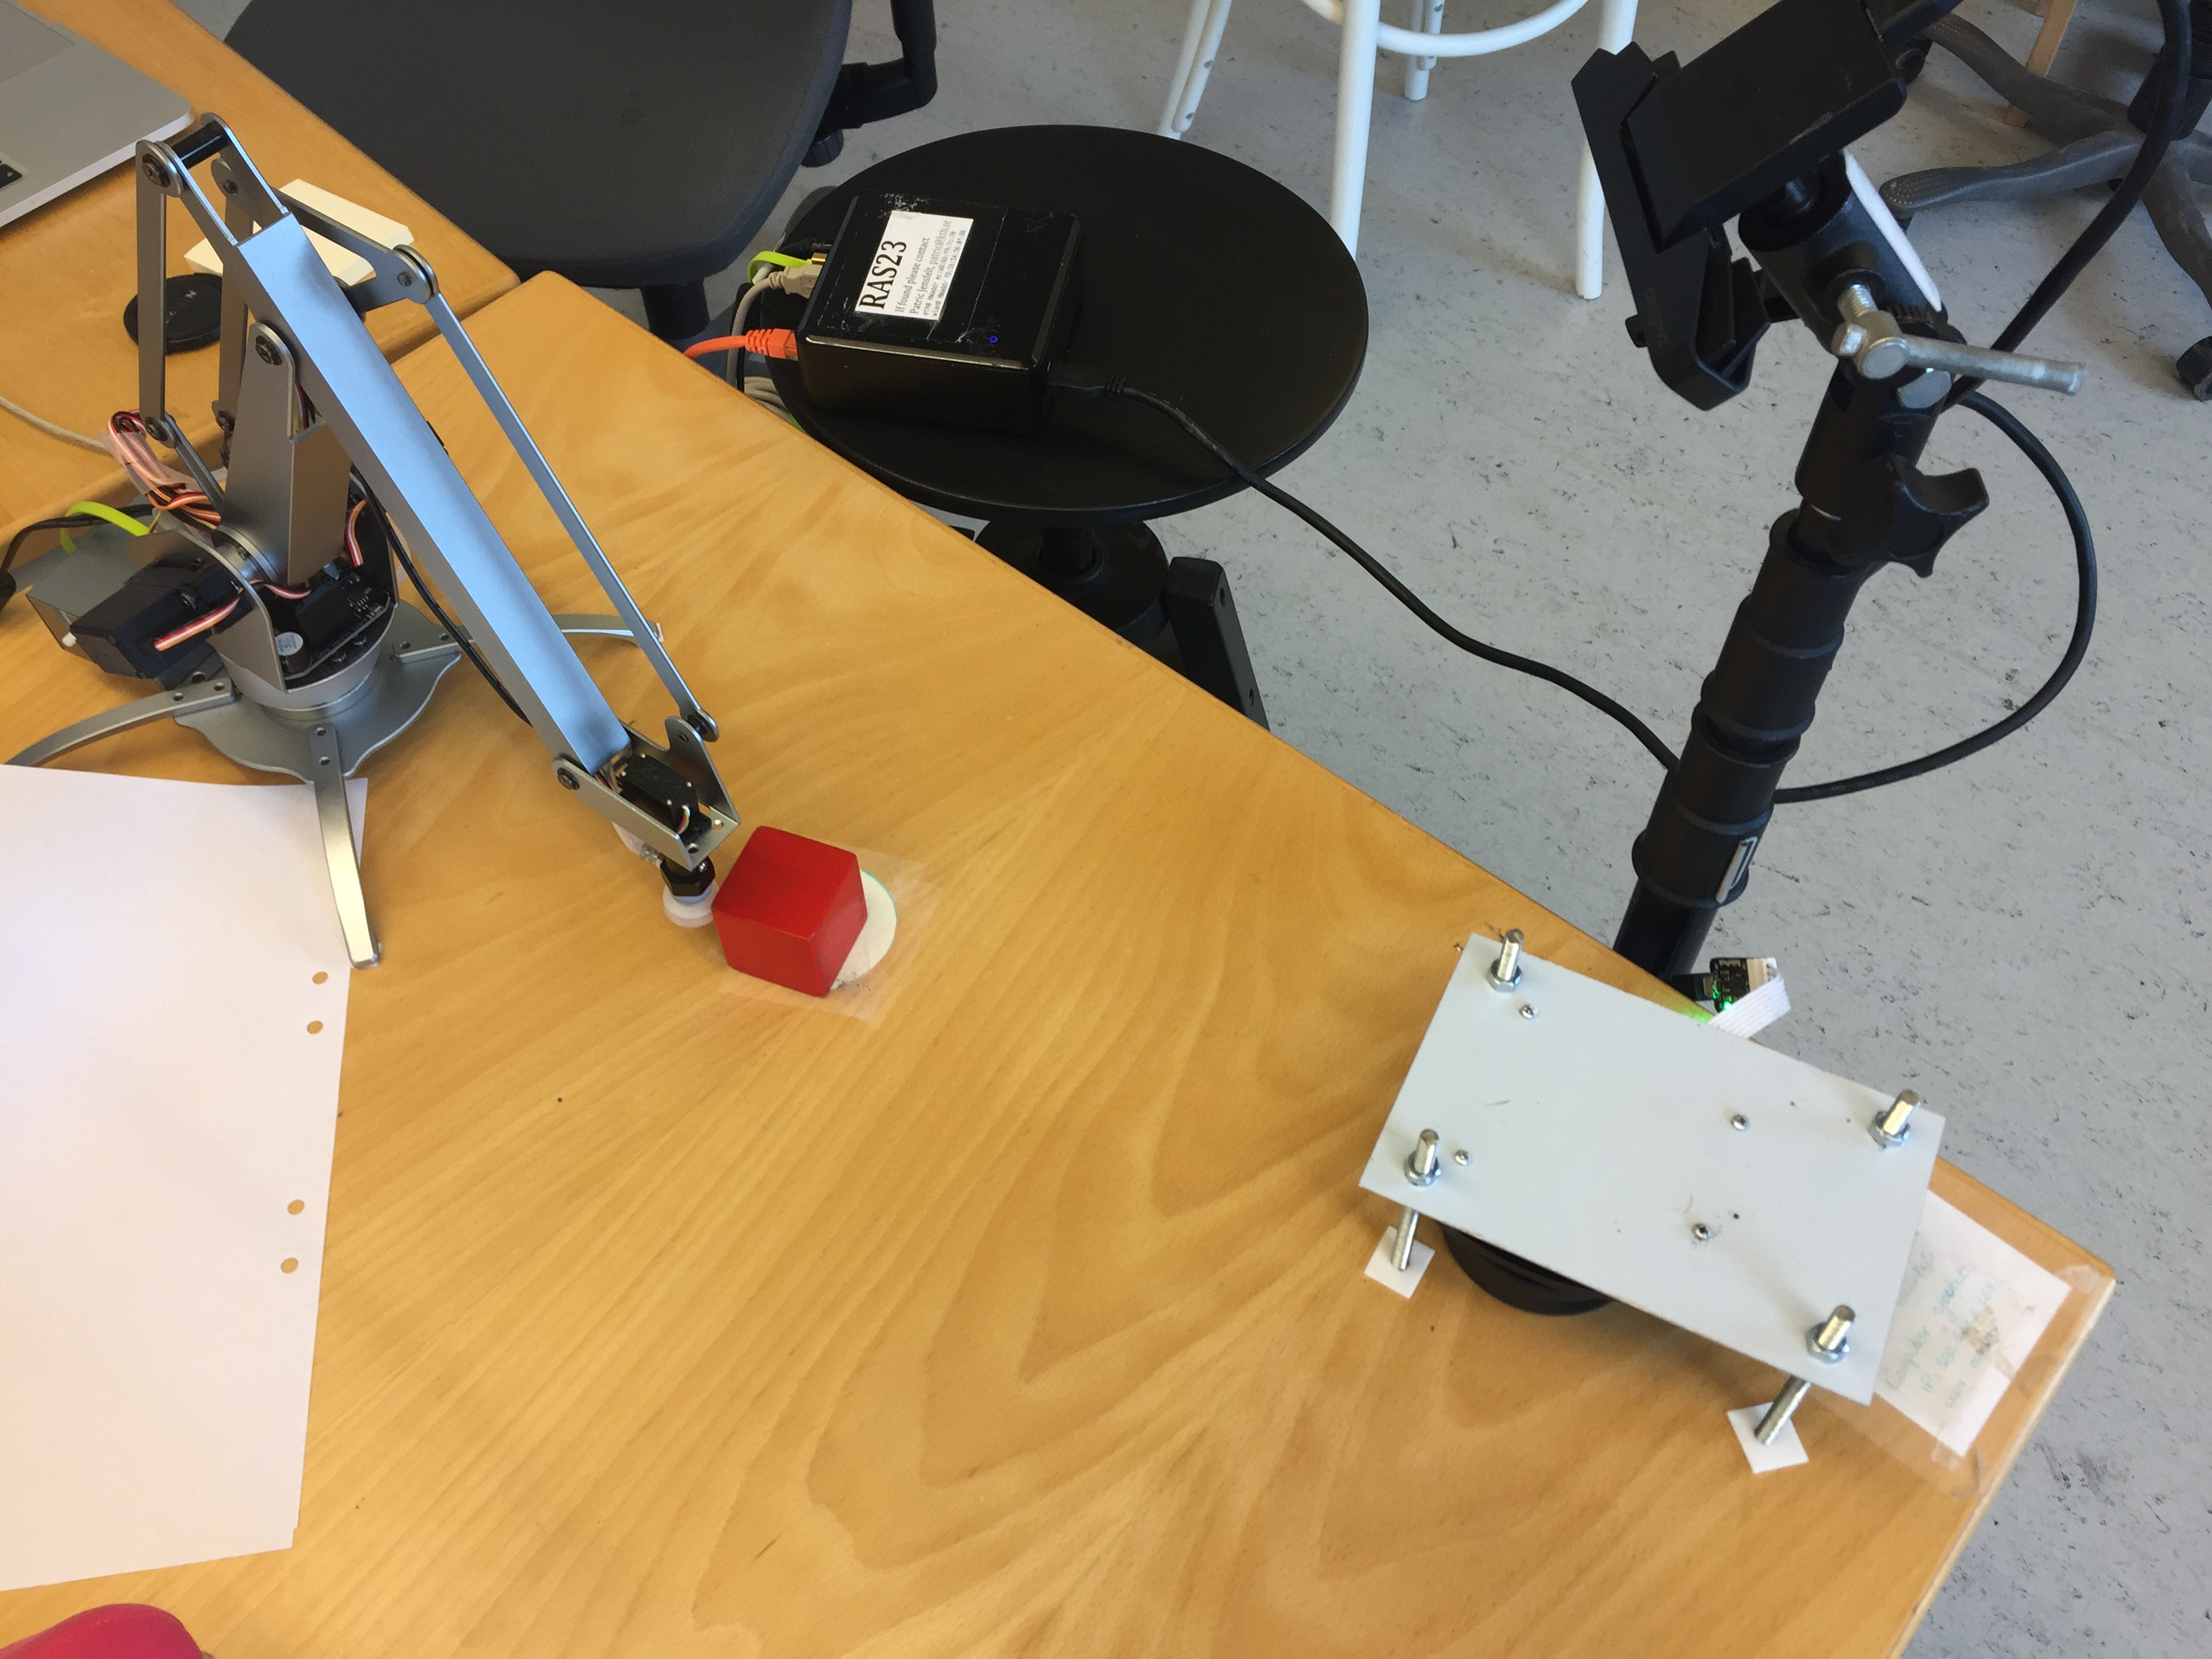
\includegraphics[width=0.4 \textwidth]{res/camera_placement_fixed.jpg}

    \caption{Fixed camera placement for pose estimation of the cube.}

    \label{fig:camera_placement_fixed}
    
\end{figure}

The first part of the network in figure \ref{fig:gps_net} was used, with two
hidden layers of 100 hidden ELU activated units each after the 2-D expected
position. The output was a 2-dimensional linear layer predicting the cube
position in the robot coordinate frame. For incorporating depth into the
network, I propose a layout, shown in figure \ref{fig:depth_net}, where depth
is input at two locations in the network. The first place is simply as a fourth
dimension into the first convolutional layer. The second place is to append the
expected distance $\mathbb{E}[D_k]$ for each feature $k \in [1, 32]$ to the
fully connected layers, using the spatial softmax as the probability when
calculating the expectation:

\begin{figure}[h!]
    \centering
    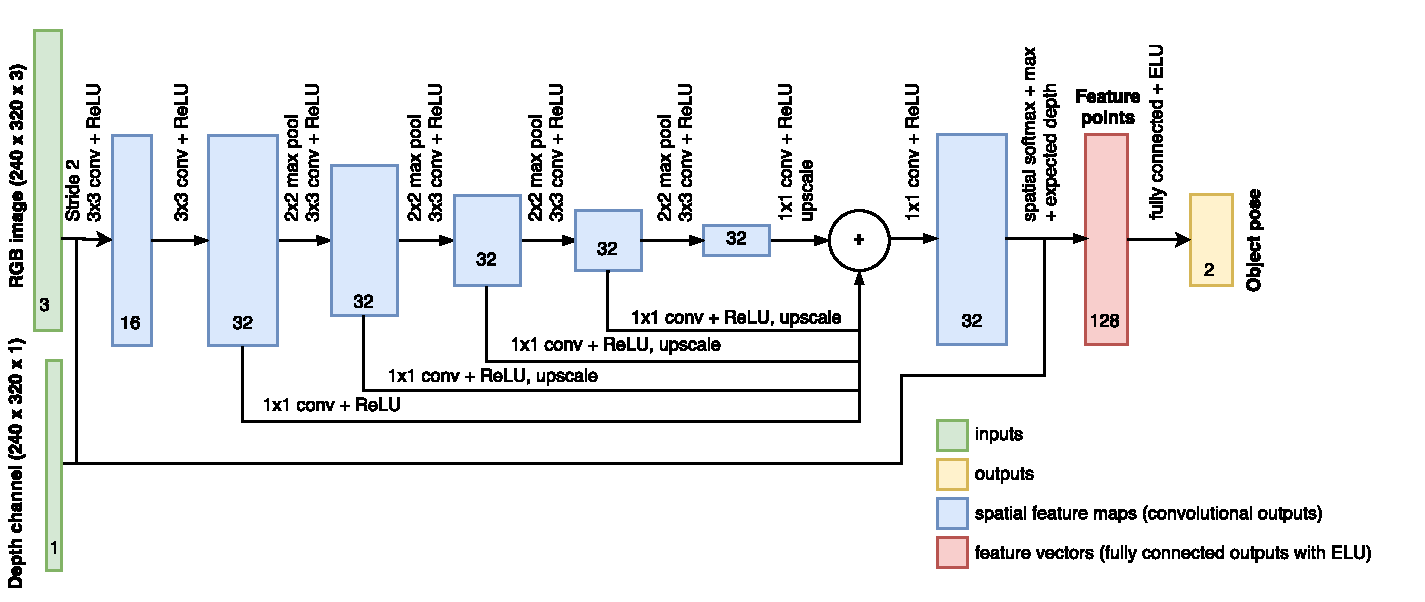
\includegraphics[width=1.0 \textwidth]{res/depth_net.pdf}

    \caption{Proposed pose estimation network incorporating depth information.
    Input to the first convolutional layer is a 4-channel RGBD image. Using the
    spatial softmax as a per-feature probability distribution, expected depths
    per feature map are also concatenated with the expectation over image
    coordinates. As a measure of uncertainty in each feature, the maximum
    activation for each feature map, after the spatial softmax, are also
    concatenated with the input to the fully connected layer.}

    \label{fig:depth_net}
    
\end{figure}

\begin{equation}
    \mathbb{E}[D_{k}] = \sum_{i, j} p(c_{i, j, k}) d_{i, j}
\end{equation}

Here, $p(c_{i, j, k})$ is the output of the spatial softmax at pixel $(i, j)$
for feature map $k$ and $d_{i, j}$ the registered depth at pixel $(i, j)$. The
network was trained by minimizing the mean square error and using the Adam
optimizer. The training and validation losses are plotted in figure
\ref{fig:depth-vs-rgb} showing that only using RGB converges faster and that
adding depth did not contribute to better scores in this experiment.

\begin{figure}[h!]
    \centering
    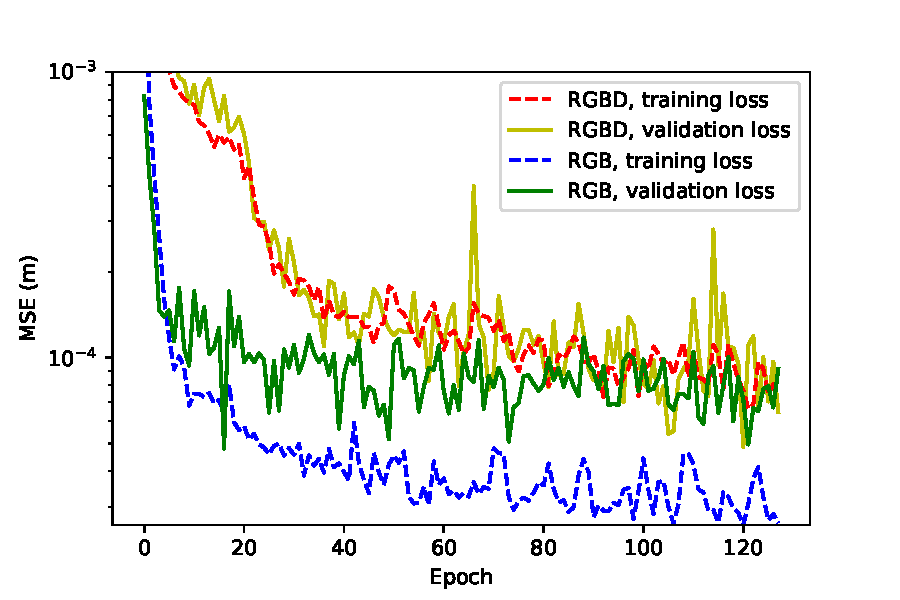
\includegraphics[width=0.6 \textwidth]{res/depth-vs-rgb.pdf}

    \caption{Training curves for pose estimation from a fixed position camera.
    Adding depth information did not lower training scores, only slowing down
    the time needed to converge.}

    \label{fig:depth-vs-rgb}
    
\end{figure}

\section{Results}

The trained network using RGB was used instead of the pose estimates from the
LIDAR and tested on a robot. The network needed significantly more time to
evaluate than when using the LIDAR estimates, the algorithm now running at 1-2
Hz compared to approximately at 10Hz using LIDAR estimates. The bottleneck when
using LIDAR estimates are not the actual LIDAR, but rather controlling the
robot and measuring servo angles etc. A video was recorded of the result and
can be seen here: \url{https://youtu.be/vakM-xvhEmE}. A dark gray cup was added
into the workspace without previous tests during recording of the video showing
that the estimation could handle some distraction. Further tests showed that
any red object will disturb the pose estimates, making the policy unsuccessful
in pushing the cube. This was expected though since no distractors were added
during data collection.

\section{Conclusions and future work}

In this thesis, NAF was evaluated in both a simulated setting and distributed
over several robots. Initial experiments with simple reaching tasks worked
fine, but extending this to a pushing task failed, even after simplifications
like keeping starting and goal positions fixed. This could either be due to
some error in the implementation that did not affect the simpler reaching task,
or that the restriction to a quadratic advantage function could not represent
the bi-modal nature of the task. DDPG however could solve this task but did not
prove stable under noisy controls and observations. Reformulation of the
problem as a partially observable Markov decision process might be an
interesting way forward since highly accurate sensors are not always what are
seen in reality.

Regarding pose estimation, a network was proposed to incorporate depth
information, a common feature nowadays even in consumer products. Simulation
showed better results when adding this feature, although for real data no
benefit was seen. Future experiments could include replacing zero representing
missing depth values with something else, for example the maximum distance
registered. Relative pose estimation was clearly shown to be capable of
learning the geometric interpretation from 2D data, although the precision was
too low for this use case. This could have been due to the neural network not
being able to represent this accurately enough, the resolution of input data or
intermediary representations being too low, or labels during training being too
noisy requiring more data for higher quality predictions. The former case is
somewhat supported by the case that simulated data giving 2D coordinates also
produced noisy estimates.


\bibliography{citations}{}
\bibliographystyle{unsrt}

\end{document}
